%%%%%%%%%%%%%%%%%%%%%%%%%%%%%%%%%%%%%%%%%%%%%%%%%%%%%%%%
% Created by Pierre Chardaire. 
% Updated by Rudy Lapeer update: 10/2024
% Final Update by Mohsin Raza Last update: 10/2025
% Change the option between square brackets
% depending on the document you have to write:
%
% review      for the literature review + plan
% progress    for the progress report
% final       for the final report
% 
%%%%%%%%%%%%%%%%%%%%%%%%%%%%%%%%%%%%%%%%%%%%%%%%%%%%%%%%
\documentclass[final]{cmpreport}


% Some package I am using. You may not need them
%
\usepackage{rotating}
\usepackage{subfloat}
\usepackage{color}
\usepackage{pdfpages}
\usepackage{url}
%\setkeys{Gin}{draft}

%%%%%%%%%%%%%%%%%%%%%%%%%%%%%%%%%%%%%%%%%%%%%%%%%%%%%%%%
%
%  Fill in the fields with:
%
%  your project title
%  your name
%  your registration number
%  your supervisor's name
%
%%%%%%%%%%%%%%%%%%%%%%%%%%%%%%%%%%%%%%%%%%%%%%%%%%%%%%%%
\title{High Speed Communication Between Raspberry Pi via Secondary Memory Interface}
%%%%%%%%%%%%%%%%%%%%%%%%%%%%%%%%%%%%%%%%%%%%%%%%%%%%%%%%
%
% The author's name is ignored if the following command 
% is not present in the document
%
% Before submitting a PDF of your final report to the 
% project database you may comment out the command
% if you are worried about lack of anonymity.
%
%%%%%%%%%%%%%%%%%%%%%%%%%%%%%%%%%%%%%%%%%%%%%%%%%%%%%%%%
\author{Charlie Flux}

\registration{100392431}
\supervisor{Gavin Cawley}

%%%%%%%%%%%%%%%%%%%%%%%%%%%%%%%%%%%%%%%%%%%%%%%%%%%%%%%%
%
% Fill in the field with your module code.
% this should be:
%
% for BIS project module   -> CMP-6012Y
% for STATS project module -> CMP-6028Y
% for CS project module    -> CMP-6013Y
%
%%%%%%%%%%%%%%%%%%%%%%%%%%%%%%%%%%%%%%%%%%%%%%%%%%%%%%%%
\ccode{CMP-7043Y}

%%%%%%%%%%%%%%%%%%%%%%%%%%%%%%%%%%%%%%%%%%%%%%%%%%%%%%%%
%
% Comment out if confidential report.
% The command should be used if the project is subjected 
% to a Non Disclosure Agreement.
%
% Three examples of the use of the \confidential command. 
% Please ask your supervisor what confidential statement 
% should be used, if appropriate.
%
%%%%%%%%%%%%%%%%%%%%%%%%%%%%%%%%%%%%%%%%%%%%%%%%%%%%%%%%
%\confidential{}

%\confidential{The contents of this report remain confidential for two years and should not be discussed or disclosed to any third party without the prior written permission from the School of Computing Sciences, the University of East Anglia}

%\confidential{The information contained in this document is confidential, privileged and only for the information of the intended recipient and may not be used, published or redistributed without the prior written consent of FruitName Ltd}

\summary{

}

\acknowledgements{
I would like to express my gratitude to my supervisor, Dr Gavin Cawley, for his support and guidance throughout the project and the engineers at Raspberry Pi for their insights and time.
}

%%%%%%%%%%%%%%%%%%%%%%%%%%%%%%%%%%%%%%%%%%%%%%%%%%%%%%%%%%%%%%%%%%
%
% If you do not want a list of figures and a list of tables
% to appear after the table of content then uncomment this line 
%
% Note that the class file contains code to avoid
% producing an empty list section (e.g list of figures) if the 
% list is empty (i.e. no figure in document).
%
% The command also prevents inserting a list of figures or tables 
% anywhere else in the document
%
% Some supervisors think that a report should not contain these
% lists. Please ask your supervisor's opinion.
%
%%%%%%%%%%%%%%%%%%%%%%%%%%%%%%%%%%%%%%%%%%%%%%%%%%%%%%%%%%%%%%%%%%
%\nolist

%%%%%%%%%%%%%%%%%%%%%%%%%%%%%%%%%%%%%%%%%%%%%%%%%%%%%%%%%%%%%%%%%%
%
% Comment out if you want your list of figures and list of
% tables on two or more pages, in particular if the lists do not fit 
% on a single page.
%
%%%%%%%%%%%%%%%%%%%%%%%%%%%%%%%%%%%%%%%%%%%%%%%%%%%%%%%%%%%%%%%%%%
\onePageLists


\begin{document}


\section{Introduction}
Modern embedded systems offer capable platforms for hobbyist and industrial applications with versatile peripheral interfaces and high-speed memory access. Among these platforms, Raspberry Pi established itself as a leading low-cost single board computer platform, offering flexibility and accessibility for both research and industrial applications. However, as hardware manufacturers move away from parallel interfaces, support for legacy parallel systems has been quietly deprecated, forcing developers to rely on additional hardware or simulations to maintain compatibility. 

This project focuses on the Secondary Memory Interface (SMI), produced by Broadcom and accessible on Raspberry Pi boards, designed to facilitate high-speed parallel memory access. Despite its unique nature, the SMI has seen limited adoption and has been described as an `unloved peripheral' in industry practice~\cite{zotero-item-18}, contributing to the lack of widespread documentation and tooling. This project's aim is twofold: first, to provide comprehensive documentation and a user-space API for the SMI on Raspberry Pi and second, to implement a functional shared memory system that demonstrates efficient data transfer between multiple processes and devices.

By combining thorough documentation and practical implementation, this project contributes both as a future reference for developers and as a practical example for high-speed shared memory usage on Raspberry Pi systems. The resulting implementation provides a platform for creating legacy support for deprecated parallel interfaces, while also encouraging further exploration of shared memory architectures on Raspberry Pi.

% This needs to be reviewed throughout the paper...
This paper presents the design, implementation and benchmarking of the Secondary Memory Interface on Raspberry Pi boards, highlighting performance differences across configurable modes and devices, in turn identifying best practices for efficient shared memory communication.

\section{Background}

\subsection{Parallel Interfaces}
The terms parallel and serial, when used to describe an interface, refers to the number of data lines used for communication. A parallel bus transmits multiple bits simultaneously across several lines whereas, a serial bus transmits data over a single line sequentially. Historically, parallel interfaces such as PCI, PATA, and external memory buses dominated computer architectures due to limitations in achievable signalling frequencies and the relative simplicity of low-frequency parallel communication across short board-level distances.

Increasing clock frequencies and system complexity gradually favoured serial interconnects such as PCI Express, SATA, and USB. Serial transmission offers several advantages over traditional parallel buses, including reduced pin count, simplified PCB routing, improved scalability and lower susceptibility signal integrity issues. Modern high-speed serial interfaces are capable of multi-gigatransfer per second data rates while minimising board area and manufacturing complexity~\cite{zotero-item-18}. As a result, many legacy parallel interfaces have been gradually deprecated in favour of serial alternatives.

Despite the widspread adoption of serial communication ports, parallel interfaces remain relevant within embedded and low-level systems where direct memory-style communication and reduced protocol overhead are desirable. Unlike packet-orientated protocols, many parallel interfaces expose simple read/write mechanics with minimal framing or encoding overhead, allowing peripherals to be accessed in a manner similar to conventional memory devices. This can significantly reduce software overhead complexity and communication latency in tightly coupled systems.

Parallel interfaces continue to be used in applications such as FPGA interfacing, memory-mapped peripherals, data acquisition systems and display controllers. In such systems, the increased pin count and routing complexity of parallel buses may be acceptable tradeoffs in exchange for predictable timing behaviour and reduced software overhead. Additionally, parallel buses can simplify direct memory access (DMA) operations by avoiding packetisation and protocol translation layers commonly associated with serial interfaces.

The Secondary Memory Interface (SMI) represents an unusual example of modern parallel interface exposed to software developers. Although originally intended for communication with external memory devices, the peripheral can be repurposed for high-throughput communication and shared-memory style interactions with external hardware. Compared to more conventional interfaces such as SPI and GPIO bit-banging, SMI offers substantially reduced protocol overhead and supports DMA-driven transfers, making it particularly attractive for embedded communication systems. However, the interface remains poorly documented and relatively unexplored within existing open-source literature, motivating further investigation into its capabilities and limitations.


\subsection{User vs Kernel Space}
% Difference between user and kernel space - why it is a good model
% Performance overhead with system calls
% Mention goal is to implement completely in user space <- Explanation on how and why in methodology
% Explain how optional kernel modules are used for the interrupts
Modern operating systems implement memory and execution privileges as a hierarchical protection model, commonly referred to as privilege rings, which partitions execution into distinct levels of hardware access~\cite{tanenbaumModernOperatingSystems2015}, providing isolation between application software and privileged system resources. Traditionally, hardware devices are controlled through kernel-space device drivers providing privileged yet controlled access to hardware resources. Executing within the kernel also allows drivers to achieve improved scheduling determinism and lower interrupt latency compared to user-space applications~\cite{minghaoPerformanceAnalysisOptimization2007}, making kernel-space implementations the conventional approach for device driver development.

Kernel-space development introduces increased engineering complexity, with faults resulting in system crashes, memory corruption and undefined behaviour hence, complicating debugging and increasing development risk. Kernel development also imposes stricter tooling and deployment requirements compared to conventional user-space software development. 

Linux provides multiple frameworks for user-space device access, including \texttt{mmap}, Userspace I/O (UIO) and the Virtual Function I/O (VFIO) subsytem. These mechanisms allow selected device memory regions to be mapped into user-space address spaces while the kernel retains responibility for previleged operations such as interrupt routing and memory management. By reducing the number of system calls required for hardware interaction, memory mapping can significantly reduce communication overhead for high-frequency I/O operations.

Despite these advantages, user-space drivers introduce several tradeoffs. User-space processes remain subject to operating system scheduling behaviour and cannot guarantee deterministic execution timing in the same manner as kernel-space implementations. Additionally, direct access to memory-mapped peripherals increases the risk of invalid hardware states if insufficient validation is performed. DMA-based communication further complicates user-space designs due to cache coherency requirements and restrictions surrounding physical memory visibility. Despite this, third-party drivers are commonly implemented in user space, utilising existing kernel interfaces to provide support for functionality overlooked or undocumented by the vendor. User-space execution additionally provides improved fault and security isolation by reducing the potential impact of compromised or untrusted software components. Recent research argues that the overhead of user-space drivers is sufficiently low that the performance penalties become negligible for many workloads compared to the increased safety~\cite{metzgerDeprivilegingLowLevelGPU2025}. Furthermore, the degree of this overhead is largely a function of kernel design~\cite{PerformanceUKernelBasedSystems}; a sufficiently mature kernel will expose an efficient enough interface surface that user-space drivers become a fully viable alternative to kernel-space implementation.

For this project, a predominantly user-space architecture was selected to simplify development and experimentation with the poorly Secondary Memory Interface. This approach reduced debugging complexity and minimised the risk of system instability during rapid iterative development while still allowing high-throughput communication through memory-mapped I/O and DMA-assisted transfers.

\subsubsection{Kernel Modules}
% What a kernel module is
Functionality is primarily loaded into the kernel at build time however, kernel modules allow functionality to be loaded and unloaded from the kernel on demand without rebooting the system, using tools such as \texttt{insmod} and \texttt{rmmod}. This flexibility makes kernel modules a practical platform for extending kernel functionality without modifying the kernel source. However, as kernel modules execute with full Ring 0 privileges, they carry the same security implications as built-in kernel code, making it desirable to keep any custom module as minimal as possible.

\subsubsection{Physical, Bus \& Virtual Addressing}
Modern operating systems abstract physical memory from user and kernel space processes through virtual addressing. Each process operates within its own isolated virtual address space, with the Memory Management Unit (MMU) transparently translating virtual addresses to physical addresses at runtime. The abstraction allows operating systems to isolate processes from one another while enabling features such as paging and protected memory regions. Consequently, the addresses observed by software applications do not directly correspond to the underlying physical memory layout.

Physical addresses represent locations within the system's main memory as viewed by the CPU and MMU. However, on many System-on-Chip (SoC) architectures, peripherals and DMA engines do not directly operate using physical addresses. Instead, hardware devices communicate using bus addresses. Bus addresses are the addresses as viewed by the SOC interconnect fabric rather than the CPU. Whilst physical and bus addresses refer to the same underlying memory, the Broadcom VideoCore MMU applies a fixed offset between the two spaces. Concsequently, a physical address and its corresponding bus address differ by a constant value. Bus addresses therefore represent the addresses that on-chip masters other than the CPU must use to correctly target a given memory address. This distinction becomes particularly important when configuring DMA transfers, as DMA controllers require bus-visible addresses rather than the virtual addresses exposed to user-space applications. Figure~\ref{bcm_address-space} outlines the relationship between virtual, physical and bus address spaces within the Broadcom BCM283x architecture.

Linux exposes mechanisms such as \texttt{mmap} to bridge this separation by allowing physical device memory regions to be mapped into user-space virtual address spaces. This enables applications to interact directly with memory-mapped peripherals while preserving kernel-mediated access control. For example, the SMI registers may be mapped into user space, allowing applications to configure transfer timings and initiate communication without requiring a fully custom kernel-space driver.

Address translation also introduces cache coherency considerations. CPU memory accesses may be cached transparently by the processor, whereas DMA engines commonly bypass CPU cache hierarchies and interact directly with system memory. Without appropriate cache management or memory synchronisation mechanisms, stale or inconsistent data may be observed between the CPU and DMA peripherals.

\subsection{Hardware Interrupt Handling}
% What hardware interrupts are
% How they are exposed to user space
% How hardware interrupts promote good user-space driver development 
Hardware interrupts provide a mechanism for peripherals to asynchronously notify the processor that an event requiring attention has occurred. Rather than continuously polling hardware devices for status changes, the processor may suspend normal execution and invoke an Interrupt Service Routine (ISR) when signalled by a peripheral. Interrupt-driven communication therefore enable more efficient CPU utilisation by avoiding unnecessary busy-waiting during idle periods.

Interrupts are widely used within operating systems for handling peripheral events such as DMA transfer completion, network packet reception and timer scheduling. Within Linux, interrupt handling is typically performed within kernel space, with user-space applications receiving notifications indirectly through kernel-managed interfaces such as file descriptors, event queues or Userspace I/O (UIO) mechanisms.

Despite their advantages, interrupts introduce execution overhead. Servicing an interrupt commonly requires context-switching, scheduler interaciton and cache disruption, all of which contribute to increased latency and reduced execution determinism. Under high-frequency workloads, excessive interrupt generation may significantly degrade system performance, commonly referred to as an interrupt storm.

Polling allows software to repeatedly monitor hardware state without relying on asynchronous notifications, potentially reducing latency and scheduling jitter at the cost of increased CPU utilisation. Consequently, may performance-critical system adopt hybrid approaches in which interrupts are used for coarse-grained event notification while high-frequency data transfer paths rely on polling or DMA-driven communication.

Within user-space driver architectures, interrupt handling introduces additional complexity due to operating system scheduling behaviour. User-space processes cannot directly service hardware interrupts and must instead rely on kernel-mediated notification mechanisms. This may increase wake-up latency compared to fully kernel-space implementations, particularly under heavy system load.

\subsubsection{Userspace I/O}
To bridge this gap, the kernel can expose interrupt events to user space through a character device, allowing user-space processes to block on a \texttt{read} or \texttt{poll} clause until an interrupt occurs~\cite{UserspaceHOWTOLinux}. This approach taken by the Linux \textit{UIO} (Userspace I/O) subsystem, which provides a standard mechanism for exposing hardware interrupts to user space via a file descriptor, enables interrupt-driven design in user space. While the security implications of custom kernel modules are well understood, the simplicity of this mechanism makes a minimal interrupt-handling module a feasible and auditable supplement to a manufacturer's existing hardware support.

For this project, interrupt-driven communication was explored alongside polling and DMA-assisted transfer mechanisms to evaluate the tradeoff between CPI utilisation, latency and implementation complexity within the SMI communication archietcture. A kernel module exposing the SMI hardware interrupt was implemented to provide event-driven notification support for user-space applications. This allowed interrupt-based synchronisation strategies to be evaluated alongside lower-latency polling approaches during high-throughput communication experiements.

\subsection{Direct Memory Access (DMA)}
% What DMA is
% Why normal transfers take up so much compute
% How we can use DMA to make software fast and do compute while we wait for it
Direct Memory Access (DMA) is a hardware mechanism that allows peripherals to transfer data directly to and from system memory without requiring continuous CPU intervention. Rather than executing explicit load and store instructions for each transfer, the processor configures a DMA controller with the source address, destination address, transfer length and transfer parameters before the transfer is executed autonomously by dedicated hardware. This significantly reduces CPU overhead during high-frequency or large-volume data transfers.

DMA is particularly advantageous within high-throughput communication systems where conventional programmed I/O would otherwise require substantial processor involvement. By offloading memory transfers to dedicated hardware, DMA allows the CPU to continue executing unrelated tasks while transfers occur concurrently in the background. This reduces software overhead, minmises interrupt frequency and improves overall system throughput compared to CPU driven memory copying operations.

Modern DMA engines commonly operate as independent bus masters capable of directly accessing system memory through the SoC interconnet fabric. Many DMA implementation support chained control blocks or scatter-gather transfers, allowing multiple transfer operations to be executed sequentially without additional CPU intervention. Such mechanisms are particularly beneficial for streaming workloads and continuous peripheral communication.

Although DMA-based communications offer several advantages compared to naive memory transfers, several engineering challenges are introduced. Since DMA engines bypass conventional CPU-driven memory access paths, memory visibility and cache coherency become important considerations. CPU memory accesses may be transparently cached, whereas DMA peripherals commonly interact directly with main memory. Without appropriate cache management or memory synchronisation, stale or inconsistent data may be observed between the processor and DMA peripherals.

DMA also complicates user-space implementations due to restrictions surrounding physical memory visibility and allocation. DMA controllers require bus-visible memory addresses and therefore cannot directly operate on arbitrary virtual memory regions allocated by user-space applications. Additionally, operating systems may relocate or page memory dynamically, making stable DMA buffer allocation non-trivial without kernel assistance or specialised allocation mechanisms.

The SMI supports DMA-paced transfers, allowing the DMA controller to operate as an independent bus master capable of autonomously transferring data between system memory and the peripheral. This reduces CPU overhead during high-throughput communication and enables more continuous transfer patterns than conventional programmed I/O approaches.

\subsection{Raspberry Pi Secondary Memory Interface (SMI)}
The Secondary Memory Interface is a parallel interface implemented by Broadcom on the BCM283x family of system on chips (SoCs), commonly found on the Raspberry Pi product range. The SMI was originally designed as an external memory bus intended to interface with slower peripheral devices that would otherwise impose performance constraints if connected directly to the primary system bus~\cite{zotero-item-12}. The interface supports configurable bus widths, programmable timing parameters and register-based peripheral communication, allowing it to interface with devices operating at substantially lower clock frequencies than the ARM system bus. Compared to conventional GPIO bit-banging or SPI-based communication, the SMI provides substantially higher potential throughput while exposing lower protocol overhead and finer timing control.

Unlike packet-orientated communication interfaces such as SPI and USB, the SMI exposes a memory-style communication model in which peripherals are accessed through direct read and write transactions. The interface hardware incorportates two asynchronous First In First Out (FIFO) buffers which regulate data transfer between the system bus and external peripherals. Data may be transferred either through direct programmed I/O operations or DMA-paced transfers, enabling high-throughput communication with relatively low software overhead. These characteristics make the SMI attractive for embedded systems requiring continuous streaming communication with external peripherals.

\subsubsection{SMI in Industry}
% Add information on the BCM SMI driver
Although the SMI is publicly referenced within official Broadcom datasheets, industry partners are often provided with additional documentation under non-disclosure agreements (NDAs). However, according to communication with Raspberry Pi engineers, this extended documentation contains little information beyond what is publicly available~\cite{zotero-item-18}. Consequently, much of the practical knowledge surrounding the interface remains fragmented across vender implementations, reverse-engineering efforts and community resources.

Despite the limited public ecosystem, industrial use of the SMI does exist. An official Broadcom NAND flash driver~\cite{nandflashdriver} demonstrates the interface in practice and has reportedly been used within legacy Roku devices to boot firmware directly from NAND flash memory~\cite{byRaspberryPiHat2021}. Such implementations demonstrate that the interface is sufficiently capable for production systems while simultaneously highlighting the scarcity of publicly accessible implementation details and reusable software abstractions.

\subsubsection{SMI in Open-Source Projects}
% Industry has limited examples
% Open source attempts: Bentham, RF Pi hat
% Why they are limited and have minimal coverage
While industry implementations are seldom publicly documented, several open-source projects have explored the SMI through reverse engineering and experimental peripheral development. One of the most significant contributions is J.~Bentham's work investigating the SMI as a high-speed parallel communication interface~\cite{iosoftcodeRaspberryPiSecondary2020}. Bentham demonstrates the feasibility of using the SMI for high-throughput ADC and DAC communication through direct register manipulation and DMA-assisted transfers. However, the implementation remains tightly coupled to specific data acquisition applications and exposes minimal abstraction for reuse within broader embedded communication systems. Furthermore, the work explicitly acknowledges incomplete understanding of portions of the SMI register interface~\cite{iosoftcodeRaspberryPiSecondary2020}, illustrating the fragmented and partially undocumented nature of the interface.

A more sophisticated, though still application-specific, implementation can be found within the CaribouLite project~\cite{CariboulabsCariboulite2026}, an open-source software-defined radio (SDR) HAT for the Raspberry Pi. Rather than directly exposing register-level access, CaribouLite introduces \texttt{smi\_stream\_dev}, a custom kernel module implementing cyclic DMA transfers and software FIFO buffering over the SMI hardware, exposing it as a standard character device. By combining DMA-assisted streaming with buffered asynchronous communication, the design enables continuous high-throughput data transfer while partially decoupling peripheral timing constraints from user-space processing latency. Despite these architectural improvements, the implementation remains strongly tailored towards SDR workloads and does not constitute a general-purpose SMI communication framework.

Collectively, existing open-source projects demonstrate that the SMI is capable of supporting high-throughput communication beyond its original intended role as an external memory interface. However, many existing implementations remain tightly coupled to specific hardware configurations and expose limited reusable abstraction. Furthermore, the sparse and fragmented state of publicly available documentation continues to impose a significant barrier to experimentation and wider adoption. These limitations motivated the development of a more general-purpose user-space communication framework capable of exposing reusable abstractions and systematic performance evaluation of the interface. 

\subsection{Dual Port SRAM}
Static Random Access Memory (SRAM) is a high-speed volatile random access memory type. Unlike Dynamic Random Access Memory (DRAM), which stores data using capacitors, SRAM is a semiconductor based implementation using flip-flop logic to store data. Therefore, SRAM is favoured in smaller cache memory due to its high cost and high speed, whereas DRAM is primarily used for a system main memory.

The interface through which a memory device interacts is accessed is referred to as a port. Single-port SRAM permits only one read or write operation at any given time, which is sufficient for architectures with a single bus master. In a shared memory architecture arbitration logic is required to maintain concurrent access between multiple devices. Dual-port SRAM addresses this by providing two independent interfaces to a single address space, with integrated arbitration logic to handle simultaneous access, making it well suited to shared memory architectures despite its high cost.

\subsection{Application Programming Interface (API) Design}
An Application Programming Interface (API) defines the boundary between a software component and its users, specifying the operations available and valid inputs \& outputs. While any functional interface technically constitutes as an API, the design of that interface has significant implications for usability, safety, maintainability and performance. A well designed API abstracts the complexity of the underlying system while exposing expansive functionality, allowing users to interact with hardware or software components without knowledge of the internal implementation.

\subsubsection{Defensive vs Contract API}
The two main philosophical approaches when designing an API are contract-based and defensive designs. Contract-based APIs make explicit promises about behaviour given valid inputs and places responsibility on the user to meet preconditions; resulting in a faster and leaner yet unforgiving API\@. A defensive API validates inputs and handles errors gracefully regardless of caller behaviour which requires a bulkier design due to additional input validation before a critical path is executed. For a hardware API the selection of philosophy is particularly consequential; an overly defensive design adds latency to every call, whilst an overly contract-based design leaves hardware state vulnerable to misuse~\cite{khlebnikovContractsUndefinedBehavior}. The appropriate balance between these approaches in the context of SMI API is discussed in the implementation chapter.

\subsubsection{Hardware APIs}
When designing a hardware API, extra caution is required as mistakes can corrupt state in ways that are difficult to recover from, unlike software exceptions which can be caught and handled gracefully. Hardware APIs are also bound by timing constraints, meaning inefficient designs can consume valuable resources or violate the timing requirements of the underlying hardware, producing undefined behaviour. 

\subsection{Shared Memory Architecture}
% Shared bus memory
% Dual port memory
Shared memory is a communication paradigm in which multiple nodes share a single common shared physical memory space~\cite{hennessyComputerArchitectureQuantitative2012}. This design allows for fast data transfers and low-latency inter-process communication~\cite{tanenbaumInterprocessCommunication2015a} without the overhead of explicit message passing or serialisation. Unlike message passing, where data must be copied across address spaces and formatted for transmission, shared memory allows a producer to write directly to a region that a consumer can read immediately, minimising latency and maximising throughput.

Shared memory architectures can be realised at different levels of the system stack. At the software level, the operating system provides mechanisms, such as POSIX shared memory, allowing processes on the same machine to share common address spaces. At the hardware level, physically shared memory devices such as dual-port SRAM extend this concept to independent processes on separate buses, providing deterministic low-latency communication without OS involvement.

A fundamental challenge of shared memory system is determining which system has logical ownership of a given address space at any point in time. Whilst hardware arbitration exists and handles bus level arbitration, preventing simultaneous electrical access to the same address, it provides no higher-level guarantee about the validity or readiness of the data it contains. A common solution is to reserve a region of the shared memory for ownership and flags or semaphores, which devices write to signal data is ready and ownership has transferred to the consuming device~\cite{tanenbaumInterprocessCommunication2015b}. The specific design ownership mechanism adopted in this project is outlined in the methodology.

\section{Methodology}
% How I approached the problem
% Decisions and reasoning 
% Maybe test bench section

\subsection{Development Stages}
% Development approach
% How problem broken down
% Key design decisions
Development followed an iterative, prototype-driven approach structured around four progressive stages, each building on the last.

The first stage was a knowledge building phase necessitated by the limited and fragmented documentation surrounding the SMI. Available sources were consolidated and register behaviour reverse engineered to establish a working understanding of the interface. An initial prototype with supporting diagnostic tooling was built in parallel to validate that understanding in practice, with findings feeding back into the documentation effort.

With a validated understanding of the hardware, the second stage progressed to the design and implementation of the SMI driver and API, abstracting register behaviour into a reusable interface. The software layer was developed and evaluated in isolation before any hardware complexity was introduced, allowing the interface to be profiled in known conditions.

The third stage validated the software stack against physical hardware, interfacing the SMI with a Lyontek LY62256 single-port SRAM module. This provided a concrete target for read and write transfers, allowing the driver and API to be exercised under real bus conditions and timing constraints before the added complexity of the dual-port shared memory system was introduced. The SMI supports bus widths of 8, 9, 16 and 18 bits, each with implications for throughput, packing behaviour and hardware compatibility. Each width was evaluated against the constraints of the system; an 8-bit bus width was selected to match the byte-addressable interface of the SRAM\@. The implications of this selection for data representation in memory are addressed in the implementation chapter.

The final stage integrated the complete software stack with the full hardware system, applying the API to the shared memory use case with the Renesas 7130SA/LA dual-port SRAM and evaluating end-to-end performance across the shared memory architecture outlined in Figure~\ref{system_architecture}

\subsection{Software Environment}
% Tools and dependencies used in context
Although the SMI driver is designed to be standalone, not requiring third-party libraries, some external dependencies were used to address challenges outside the core scope of the project.

\subsubsection{u-dma-buf}
A fundamental challenge of user-space DMA is cache coherency; the CPU and DMA controller hold independent views of memory and without explicit coherency guarantees, data written by one may not be visible to the other subsequently producing undefined behaviour. The CPU caches frequently accessed memory in L1/L2 cache to avoid slow main memory accesses whereas the DMA controller bypasses the cache entirely. When the CPU writes data, it may remain in the cache and not be flushed to main memory immediately hence the DMA controller may read stale data that the CPU has not flushed yet. Equally, the DMA controller may write data to the main memory which may not be visible to the CPU if it holds a cached copy of that address range. u-dma-buf~\cite{ichiroIkwzmUdmabuf2026} is a kernel module that allocates physically contiguous, cache-coherent memory regions and exposes them to user space via a device file, resolving this issue without requiring a custom kernel module.

The SMI driver is designed to accept a DMA buffer address directly, decoupling it from any specific allocation mechanism, a flexibility that aligns with the open-source nature of the project. Therefore, u-dma-buf is not a hard dependency; any cache-coherent physically contiguous buffer is sufficient. However, u-dma-buf was chosen as it provides the most straightforward means of obtaining such a buffer in user space and is used consistently throughout development for this reason.
A fully featured DMA library was considered, but such libraries typically abstract buffer management in a way that conflicts with the driver's design of accepting a raw buffer address. Additionally, the SMI driver requires simple DMA controller functionality and would not take full advantage of an external DMA library. u-dma-buf was preferred as it resolves the allocation and coherency problem while remaining transparent to the driver.

\subsubsection{Build Configuration}
The driver is built using the GNU Compiler Collection (GCC) with a provided Makefile, compiled against the C11 standard with POSIX extensions enabled via \texttt{D\_POSIX\-\_C\_SOURCE=199309L}. The highest level of compiler optimisations were enabled via \texttt{-O3} and \texttt{-march=native}, allowing the compiler to take full advantage of the native instruction set of the target platform. All levels of optimisation were tested however, \texttt{O3} was chosen to remove any computational bottleneck and allow a full evaluation of the interface.

A set of driver-specific preprocessor directives are passed via \texttt{SMIFLAGS}. Most notably the Pi model flag (e.g. \texttt{-DPI3} or \texttt{-DPI4}) is a required build argument that determines the physical base address, which differs between Raspberry Pi models. Omitting this flag will produce a compile-time error. Optional flags include \texttt{-DSMI\_VERBOSE} to enable diagnostic logic and \texttt{-DSMI\_COLOURFULL\_ERRORS} to enable colour-coded error output, both of which are useful during development and debugging but can be omitted for production builds.

The Makefile separates source files into driver modules and application code, compiling each unit independently into a dedicated build directory before linking.

\subsection{Secondary Memory Interface Modes}
% Explain each SMI mode
% Which modes were used
The Secondary Memory Interface (SMI) has a wide range of configurations, notably multiple bus widths, offering 8, 9, 16 and 18-bit modes, each with implications for throughput and hardware compatibility. Each mode was tested in isolation and evaluated against the constraints of the system, namely the interface width of the dual-port SRAM\@. An 8-bit bus width was chosen due to the byte-addressable SRAM used in the final design. The selected bus width additionally has implications for how data is represented in memory, which is addressed in the implementation chapter.

\subsection{System Design}
% Describe the overall architecture
% How each component connects to each other
Figure~\ref{system_architecture} outlines the shared memory architecture implemented. The system contains two Raspberry Pi single board computers interfacing a dual port SRAM shared memory via the SMI interface. To expand the address space available, dedicated loadable page address registers were also implemented to occupy the upper byte of the address with the lower 6 bits coming from the dedicated SMI address bus. As the page address registers are asynchronous to the SMI address bus, crossing a page boundary will add latency to read/write accesses during operation. Memory ownership is managed via a reserved flag region in the SRAM that signals data readiness and transfers logical ownership between devices.

\subsection{Hardware Setup}
% Physical wiring
% Any PCBs used or created
Prototyping was completed on a breadboard due to their simplicity and ease of rapid prototyping. During testing issues with signal integrity on breadboards imposed constraints on the timing configuration however, the setup provided a proof of concept that could be used for SMI debugging. These issues were addressed during the final implementation with all components being soldered to individual printed circuit boards (PCBs). Jumper wires were used to interconnect the PCB modules which maintained modularity and simplified debugging. The page address registers used Texas Instruments 74HC193 4-bit counters for their asynchronous incrementing and load operations.

\subsection{Benchmark Environment}
% Optional? If there is enough content to justify it


\section{Implementation}
% What was actually built
% Software implementation & hardware implementation sections
% API design etc...
The implementation was designed as a layered communication framework exposing progressively higher levels of abstraction over the Raspberry Pi SMI. At the lowest level, the system provides direct access to memory-mapped SMI registers and DMA configuration primatives. Higher layers build upon these foundations to expose transfer abstractions, buffering mechanisms, timeout handling and user-facing APIs suitable for communication with peripherals. The implementation prioritised low overhead, modularity and experimental flexibility while minimising kernel-space complexity wherever possible.

The hardware implementation consisted of simple breakout boards for the SRAM and page address registers, with decoupling capacitors to stabilise the supply voltage. The primary implementation complexity therefore lies in the software layer.
\subsection{Hardware Implementation}
The hardware implementation consisted of simple breakout boards for the SRAM and page address registers, with decoupling capacitors to stabilise the supply voltage. 

\subsection{SMI Hardware}
Figure~\ref{smi_block_diagram} illustrates the internal architecture of the SMI hardware. At its core, two asynchronous FIFOs ($64 \times 32$-bit) bridge the AXI clock domain and the SMI clock domain, decoupling the system bus from a slower peripheral clock. Write data from the AXI slave is pushed into the transmit (TX) FIFO and then drained on to the SMI data bus, whilst incoming data from the SMI bus is captured into the receive (RX) FIFO and read back up via the AXI slave. The data format block handles the bus width configuration (8, 9, 16 and 18-bits) and the RX packing which allows received data to be packed into 16-bit RGB565 or 32-bit XRGB format furthermore, the data format block can swap the received word's bit order. External DMA requests may be passed through the top two bits of the data bus as paced by the DMA control block. The Transfer Timing Mode Select block generates external bus control signals such as the read and write strobe \texttt{SOE\_N/SE} and \texttt{SWE\_N/SRW\_N}, which are physical signals used to trigger read and write operations on the connected peripheral. The interrupt control block monitors FIFO status and asserts relevant interrupt signal \texttt{o\_smi\_int} such as transfer completion or FIFO level threshold events. The 6-bit address bus \texttt{o\_smi\_addr} carries the device address to the external peripheral however, it can be repurposed as a general-purpose parallel output.

On the BCM283x, all peripherals are controlled through memory-mapped registers residing at fixed physical addresses within the peripheral address space. An example register can be seen in Table~\ref{dcs_register}. 

The SMI can be programmed to carry out a sequence of transfers to a given address ahead of time (programmed transfer) or can be completed individually (direct transfer). Direct transfers are controlled via the direct control registers: Direct Control and Status \texttt{DCS}, Direct Address \texttt{DA} and Direct Data \texttt{DD}. Programmed transfers are controlled via the SMI registers: Control and Status \texttt{CS}, Length \texttt{L}, Address \texttt{A} and Data \texttt{D}. Programmed transfers can also be paced via DMA, controlled by the SMI DMA Control \texttt{DC} register. There are four SMI device settings that can be stored by Device Read Settings \texttt{DSR} and Device Write Settings \texttt{DSW} registers which are then selected at transfer configuration time in the \texttt{A} and \texttt{DA} registers.

\subsection{Software Implementation}
Figure~\ref{software_architecture} shows layered architecture of the software implementation, built from the ground up, exposing a general-purpose API to the end user. Each layer is designed to be as thin as possible, delegating complexity upwards and maintaining a clear separation of concerns. Whilst the top-level SMI API is intended for general use, the underlying layers are independently accessible, allowing users to bypass higher-level abstractions and build custom functionality directly on top of the lower layers if required. This modularity is a deliberate design principle, consistent with the open-source nature of the project. All code was written in C, consistent with the system programming requirements of the project and the language conventions of the Linux kernel ecosystem.

\subsection{SMI Kernel Module}
The SMI kernel module is an optional module that exposes the SMI's hardware interrupt to user-space via a character device, allowing user-space processes to block on a \texttt{read} or \texttt{poll} call until a transfer-complete interrupt is asserted.

The interrupt handle \texttt{smi\_handler} is registered to IRQ 90, the BCM283x SMI interrupt line, via \texttt{request\_irq}. On each invocation, the handler reads the \texttt{SMI\_CS} register and inspects the \texttt{DONE} flag. If asserted, the flag must be cleared by writing it back, an atomic interrupt counter is incremented, and any processes blocked on the wait queue are woken. An atomic interrupt counter was required since \texttt{smi\_handler} executes in interrupt context whilst the \texttt{read} and \texttt{poll} file operations execute in process context, a non-atomic counter introduced a data race between the two execution contexts.

The module registers a character device \texttt{smi\_irq}, exposing two file operations: \texttt{read} and \texttt{poll}. Blocking on \texttt{read} suspends the calling process until the interrupt counter is positive, at which point the counter is decremented and the call returns, consuminmg one interrupt event. The \texttt{poll} implementation register the process with the wait queue, allowing the interrupt event to be multiplexed alongside other file descriptors using \texttt{select} or \texttt{poll} without blocking. Together these interfaces support both a simple blocking model and a non-blocking event-driven model, depending on the concurrency requirements of the calling application.

The module's sole responsibility is translating a hardware interrupt into a file system visible event, keeping the kernel-space footprint as small as possible and the security audit surface minimal. The IRQ number is hardcoded as a preprocessor definition rather than resolved dynamically from the device tree via; whilst the latter is the architecturally correct approach for a production implementation, it requires device tree authorship that is outside the core scope of the project, and the fixed IRQ is sufficient for reliable operation on the narrowly defined target hardware.

\subsection{SMI Driver}
The SMI driver is the lowest level of implementation that interacts with the SMI registers. Functionality is split into modules, each accompanied by a matching header file, separating the public interface from the internal implementation. Whilst both the low-level driver functionality and high-level API are implemented within \texttt{smi.c}, they are discussed separately to reflect their distinct roles in the software architecture.

\subsubsection{SMI Context Struct}
Rather than relying on global state, all register mappings, device configurations and buffer references are encapsulated within a context structure \texttt{SMI\_CXT}, allowing multiple independent instances to coexist and making the driver's dependencies explicit at every call site. Context structs can be initialised and refreshed using helper functions such as \texttt{smi\_init\_\-cxt\_\-map} to map peripheral registers and \texttt{smi\_sync\_\-context\_\-device} to synchronise the device timing configuration with the current context state.

\subsubsection{Register Representation}
All registers can be represented as 32-bit unsigned integers however, raw integer manipulation requires complex bit-masking and shifting that obscures the intent of each operation. SMI registers are therefore represented using a union of a named bitfield struct and a raw \texttt{uint32\_t}, allowing registers to be accessed by name whilst retaining the ability to read or write the entire register atomically. 

Bitfield layout is not guaranteed by the C specification and is left to compiler discretion, making bitfield-based register representation non-portable in the general case. However, as the driver is specifically targeting BCM283x processors, the GNU Compiler Collection (GCC) is the de facto compiler for this platform. Under GCC on ARM, bitfield ordering is well defined and consistent, making this a safe and pragmatic design choice within the constraints of the system.

Each bitfield member is declared \texttt{volatile} to prevent the compiler from optimising away hardware register accesses, ensuring every read and write produces an actual memory transaction. The bitfield struct is declared with \texttt{\_\_attribute\_\_((packed))} to prevent the compiler inserting padding between members during optimisation, ensuring the in-memory layout corresponds exactly to the hardware register specifications. Furthermore, registers are aligned to 4-byte boundary using \\ \texttt{\_\_attribute\_\_((aligned(4)))}, ensuring that register accesses are never split across word boundaries, which would produce undefined hardware behaviour on the BCM283x memory bus.

\subsubsection{Transfer Modes}
The driver exposes two transfer modes: direct transfers, which execute a single read or write operation immediately via the \texttt{DCS}, \texttt{DA} and \texttt{DD} registers, and programmed transfers, which configure the SMI to execute a sequence of transfers to a given address via the \texttt{CS}, \texttt{A}, \texttt{D} registers. Each mode is exposed through single and array variants, for example \texttt{smi\_direct\_read} and \texttt{smi\_direct\_read\_arr}, providing a consistent interface regardless of transfer length. Each transfer mode is paired with a corresponding await function, such as \texttt{smi\_read\_await} and \texttt{smi\_read\_await\_direct}, which block until the transfer completes.

% During implementation of the transfer functions, the \texttt{CS} register status flags were found to be inconsistent with the documentation~\cite{zotero-item-12}. Specifically the RX and TX flag names are swapped; \texttt{rxd} in the documentation describes the RX FIFO data availability, whist the \texttt{txd} describes the TX FIFO data availability


\subsubsection{Timeout Handling}
To handle variable hardware latency without wasting processor cycles unnecessarily, await functions employ a tiered spin strategy. The system progressively trades responsiveness for CPU efficiency as the wait grows longer. This approach ensures high-performance, low-latency communication for fast operations while minimising CPU utilisation during extended stalls. Figure~\ref{timeout_strat} outlines the tiered strategy implementation and interaction between timeout handler, CPU and operating system scheduler.

The waiting logic transitions through four distinct tiers based on the incrementing spin counter. The first tier performs active polling, continuously monitoring the hardware state without interruption, keeping the CPU pipeline hot and ensuring the lowest possible response latency upon state transition. Once the spin counter exceeds the hard limit, the second tier inserts a \texttt{yield} instruction accompanied by a compiler memory barrier, hinting to the CPU that the thread is in a spin-wait loop and preventing load/store reordering without surrendering the thread's scheduler quantum. Beyond the malleable limit, the third tier invokes \texttt{sched\_yield}, instructing the OS scheduler to move the thread to the end of the run queue for its current priority level, allowing other taks to execute while the thread remains runnable. For extended delays beyond the soft limit, the fourth tier invokes the POSIX \texttt{nanosleep} interface, blocking the calling thread and fully releasing the CPU core to the kernel until the specified interval elapses.

The thresholds governing tier transitions are compile-time configurable via preprocessor definitions, allowing the spin behaviour to be tuned for different hardware characteristics without modifying the driver logic. The tier transitions were determined empirically by profiling transfer completion spin counts across a range of operating conditions. Measurements were taken both idle and loaded system conditions to characterise the boundary between hardware latency and OS scheduling jitter.

\subsubsection{DMA Transfers}\label{sec_dma_transfers}
Programmed I/O transfers require the CPU to continuously service the SMI FIFO by explicitly reading or writing individual words through the interface registers. Under sustained workloads this become increasingly inefficient, as the processor must repeatedly poll FIFO state while competing with other tasks for scheduler time. To reduce CPU overhead and improve transfer scalability, support for DMA-paced transfers was implemented using the BCM283x DMA controller.

DMA transfers allow data movement to occur independently of the CPU by configuring the DMA engine to transfer data directly between memory and the SMI FIFO. Transfer behaviour is described through DMA Control Blocks containing the source address, destination address, transfer length and pacing configuration. Once configured, the DMA engine operates autonomously, issuing memory transactions without requiring further CPU intervention until transfer completion.

Figure~\ref{dma_flow} illustrates the DMA transfer path implemented by the driver. For write transfers, data is copied into a DMA-visible buffer before being streamed directly into the SMI transit FIFO. Read transfers operate universly, with data captured from the SMI receive FIFO into the DMA buffer before being unpacking into the final application-visible representation.

The SMI peripheral exposes DMA request (DREQ) signals allowing transfers to be hardware paced accoring to FIFO occupancy. The DMA controller therefore only advances transfers when sufficient FIFO space or data availability exists, preventiong FIFO underflow or overflow conditions without requiring continuous software polling. DMA pacing thresholds are configured through the \texttt{DC} register independently for both read and write directions.

DMA operation additionally introduces memory coherency considerations. CPU memory accesses are ordinarily cached transparently by the ARM cores, whereas the DMA controller accesses system memory directly through the SoC interconnect fabric. Consequently, memory modified by the CPU may not immediately be visible to the DMA engine if the corresponding cache lines have not been written back to main memory. Likewise, data written by the DMA engine may not be visible to the CPU if stale cache lines remain resident within the processor cache heirachy. To avoid these coherency issues, DMA transfers utilise cache-coherent memory allocated through \texttt{u-dma-buf}. The allocated buffer is simultaneously accessible by both the CPU and DMA controller while remanining coherent across both execution domains.

The coherent buffer and associated DMA metadata are tracked within the \texttt{SMI\_CXT} structure. For write transfers, the DMA Control Block source address is configured to the buffer's bus-visible address while the destination is configured as the bus address of the SMI \texttt{D} register. REad transfers reverse this configuration, using the SMI data register as the DMA source and the coherent buffer as the destination.

DMA-assisted transfers substantially reduce CPU utilisation during sustained communication workloads, particularly under scheduler contention where programmed polling-based transfers may otherwise monopolise processor time. Ther performance characteristics and scheduler interactions of DMA-paced communication are evaluated further in Section~\ref{sec_results_and_eval}.

\subsubsection{Packing \& Unpacking}
The SMI FIFO interfaces with the AXI bus which operates on 32-bit words regardless of the configured SMI bus width. As a result, all data passing through the FIFO is padded to 32-bit width, meaning an 8-bit transfer consumes a full 32-bit FIFO entry. To mitigate this inefficiency, the SMI hardware supports optional packing modes which consolidate multiple bus-width samples into a single 32-bit FIFO entry. Data may be packed into either 16-bit RGB565 or 32-bit XRGB format, as illustrated in Figure~\ref{8_bit_pack}, reducing the number of memory transfers required by up to $4\times$ in the case of 8-bit RGB565 packing and significantly improving transfer throughput.

When packing is not enabled, received words are truncated to the configured bus width via the \texttt{smi\_truncate} family of functions, discarding the unused upper bits of each 32-bit word. When packing is enabled, the more complex unpacking process is required to reconstruct the original samples from the consolidated FIFO words.

Unpacking function selection is managed through the \texttt{SMI\_CXT} context, which dispatches the appropriate unpacking function based on the configured bus width and pixel format. Each bus width and format combination has a dedicated unpacking function, with performance-critical word-level operations implemented as \texttt{static inline} functions to eliminate function call overhead in the hot path. Lookup-table based unpacking was evaluated during development but ultimately rejected due to the limited L1 cache capacity of BCM283x processors. Cache misses incurred greater latency than the equivalent branch-based unpacking logic, making the reduced instruction count insufficient to offset the additional memory access overhead. The SMI also has the ability to swap the bit order FIFO words to support little-endian peripherals. Dedicated swap variants are provided for each unpacking function to handle this configuration.

Data written to the TX FIFO can also be packed, instructing the SMI controller to unpack the 32-bit FIFO values into sequential transfers.

% During implementation, the 18-bit RGB565 and XRGB unpacking swap variant modes were found to produce data with an unexpected bit order that could not be reconciled with the available documentation. Whilst non-swapped variants were successfully implemented, the correct unpacking scheme for 18-bit swap packed data could not be definitively determined. This remains an open limitation of the current implementation and is discussed further in the conclusion.

\subsection{Transfer Design}

\subsubsection{Buffer Management}
When packing is enabled, an intermediary buffer is required to temporarily store raw FIFO data before unpacking, as the unpacking functions operate on 32-bit words rather than individual samples. Buffers may be allocated either on the stack, which offers the lowest allocation overhead but is constrained by the finite stack size, or on the heap, which incurs allocation overhead but can accommodate significantly larger allocations. For small transfers, stack allocation is sufficient and avoids heap allocation overhead entirely. However, as transfer sizes grow, stack allocation becomes impractical and risks a stack overflow, necessitating heap-based allocation. To handle this transparently, the transfer functions manage an internal heap-allocated buffer tracked within \texttt{SMI\_CXT}. When a transfer is requested that exceeds the current buffer capacity, \texttt{realloc} is used to grow the buffer to the required size. The buffer is retained across calls, growing lazily to the high watermark of the largest transfer issued during the lifetime of the context, avoiding repeated allocation overhead for transfers of similar size. The buffer can be manually resized to save space between transfers using provided helper functions and is freed entirely when the context is destroyed via \texttt{smi\_unmap\_cxt}.

The threshold below which stack allocation is used and above which heap allocation is triggered is user configurable, allowing the trade-off between stack usage and heap allocation overhead to be tuned for the target application. This design ensures buffer management is handled transparently by the driver without imposing a fixed memory policy on the caller.

\subsubsection{Transfer Chunking}
Issuing a single large programmed transfer is suboptimal due to FIFO saturation and bus contention that accumulates over the duration of the transfer. To address this, a chunking mechanism was implemented that subdivides a large transfer into a sequence of equally-sized blocks, each dispatched via a separate call to \texttt{smi\_prog\-rammed\_read}. The block size is user-configurable, allowing transfers to be tuned for the target hardware and operating conditions.

For a transfer of $N$ samples with a configured block size $B$, the transfer is split into $\lfloor N/B \rfloor$ full blocks with any remaining samples handled in a final partial block, ensuring the complete transfer is issued regardless of whether $N$ is evenly divisible by $B$. The optimal block size is dependent on the bus width and packing mode in use, as these affect the number of 32-bit FIFO entries required per sample. The performance implications of transfer chunking across all supported bus widths and packing modes are evaluated in Section~\ref{sec_results_and_eval}

\subsubsection{Automatic DMA Threshold}
% Needs to be completed with the final implementation details
A natural extension of the chunking mechanism is to automatically select DMA-paced transfers above a configurable transfer size threshold, mirroring the approach taken by the Linux kernel for its own DMA subsystem. Below the threshold, programmed transfers are used directly; above it, the DMA controller is engaged to offload the transfer from the CPU\@. This reduces CPU utilisation during large transfers and is particularly beneficial under a busy scheduler, as discussed in Section~\ref{sec_dma_transfers}.

\subsection{API Design}
The API layer is built directly on top of the SMI driver, exposing a general-purpose interface for SMI communication. A deliberate distinction is made between the public-facing API and internal worker functions in terms of input validation and philosophy. 


% The two principle philosophises when designing an API are defensive and contract-based design. A defensive API pre-empts potential failures through input validation and error handling, producing meaningful error codes on failure regardless of caller behaviour. A contract-based API instead requires the caller to satisfy a set of preconditions before invoking a function, with the function guaranteeing a set of postconditions in return. This approach assumes the caller obeys the contract, places responsibility on the caller rather than the function. Both approaches have valid use cases; however, defensive APIs are often criticises for increasing code complexity and introducing runtime overhead that is particularly undesirable in performance-critical paths~\cite{khlebnikovContractsUndefinedBehavior}.

\subsubsection{API Implementation}
Both defensive and contract-based design present trade-offs that are particularly consequential for a hardware API. The SMI API adopts a hybrid approach, applying each philosophy where it is most appropriate within the software architecture. Public-facing interfaces such as \texttt{smi\_direct\_read} and \texttt{smi\_programmed\_read} adopt defensive design, validating inputs and returning error codes on failure to ensure safe usage at the API boundary. Internal worker functions, including the await and unpacking routines, adopt contract-based design, assuming valid inputs as a precondition and eliminating redundant validation from performance-critical paths. The hybrid approach ensures safety at the public interface without compromising the performance of internal transfer and unpacking operations. Furthermore, the open-source nature of the driver encourages users to build their own abstractions directly on top of the lower-level interfaces, leveraging the contract-based internals where performance is a priority.

\subsection{SMI Lite}
\texttt{smilite.h} is a single-header implementation of the SMI driver designed for users who require a lightweight integration path without the overhead of the fill multi-file driver. Single-header libraries are a common pattern in C development, allowing entire implementation to be included into a project by adding a single \texttt{\#include} directive, eliminating the need for a separate compilation step or build system integration.

\texttt{smilite.h} includes the complete register definitions, memory mappings utilities, address translation macros, timeout handle, await routines and the full suite of unpacking and truncation functions. However, it deliberately omits the higher-level initialisation helpers such as \texttt{smi\_init\_cxt\_map} and \texttt{smi\_init\_rw\_config}, leaving peripheral setup and context initialisation to the user. The user must also define system specific macros, most notably \texttt{PHYS\_REG\_BASE} which specifies the physical register address base which differs across BCM283x variants, enforced at compile time via a preprocessor error. These requirements makes the platform dependencies explicit rather than silently assuming a specific hardware configuration, improving portability across BCM283x variants.

\subsection{Implementation Limitations}


\subsection{Shared Memory Implementation}

\section{Results and Evaluation}\label{sec_results_and_eval}
All measurements were conducted on stock Raspberry Pi hardware under idle system conditions, with no modifications to device specifications or kernel parameters. Each configuration was evaluated using a transfer size of $1,048,576$ bytes (1 MiB), preceded a single warmup run to ensure hardware and cache state were stable before measurement. Five timed measurements were then recorded per configuration, with the reported throughput representing the mean of these five runs.

The driver was compiled with GCC at the \texttt{O3} optimistaion level for all measurements, with \texttt{march=native} enabled to allow the compiler to take advantage of the native instruction set of target platform. To characterise the impact of compiler optimisation on transfer performance, one configuration was additionally evaluated across all GCC optimistaion levels.

To isolate the performance of the SMI interface itself, measurements were taken without any peripheral connected, eliminating any bottleneck introduced by peripheral access latency. Results are presented for both the Raspberry Pi 3B+ and Raspberry Pi 4, across all supported bus widths, packing modes and transfer types, with block size ranging from $8$ to $1,048,576$ bytes. Transfer duration was measured using \texttt{clock\_gettime} with the \texttt{CLOCK\_MONOTONIC} clock source, which provides nanosecond resolution and is immune to system time adjustments. As wall clock time is measured rather than CPU time, OS scheduling jitter represents a potential source of variance; idle system conditions and multiple run averaging were used to minimise this effect. Throughput is reported in both megbits per second (MB/s) and megatransfers per second (MT/s) to account for the differing data widths across bus width and packing mode configurations. The SMI clock was also run at its fastest with 2ns divisions. A transfer is defined complete once the data is its target format therefore, packed transfers must be unpacked before the transfer is complete.

% Add more for this above and below. Calculate clock speed.
Visualistaions log scale the $x$ axis when necessitated.

Due to hardware failure of the Raspberry Pi 4 during testing, a complete dataset could not be obtained for all configurations on that platform. Where Raspberry Pi 4 data is unavailable, results are presented for the Raspberry Pi 3B+ only, with noted comparisons between platforms where data permits.

\subsection{Throughput Results}

\subsubsection{Non-Packing Transfers}
Figure~\ref{3b_throughput_mts_nopacked} shows that all bus widths achieve similar transfer rates, peaking just under 9 MT/s. This convergence is expected as MT/s measures the number of transfers per second regardless of bus width as each transfer consumes one FIFO entry irrespective of how many bits it carries. Performance degrades significantly for block sizes under $10^3$ bytes, where per-transfer software overhead dominates over the transfer itself. A slight performance reduction is observed for block sizes exceeding $10^5$ bytes across both packed and non-packed configurations. The precise cause is difficult to isolate, however working backwards from the hardware specification of the Raspberry Pi 3B+ we can make educated guesses to the cause. Figure~\ref{3b_cache_misses} comparing the L1 cache misses against block size showing the spike in misses as the block size approaches the Raspberry Pi 3B+ L1 data cache size of 32KB, then drops once higher level caches are prioritised for data storage. Figure~\ref{3b_cache_misses_throughput} overlays this data with Figure~\ref{3b_throughput_mts_nopacked}, showing a plausible correlation between the cache miss rate and transfer throughput as higher level caches are used instead of the smaller but faster L1 cache. This degradation is almost nullified on the Raspberry Pi 4, consistent with the larger cache, faster memory subsystem and improved Translation Lookaside Buffer handling sustaining performance at greater block sizes. Figure~\ref{3b_throughput_mbs_nopacked} reveals the effect of bus width on effective data throughput; the 18-bit configuration achieves approximately 19 MB/s, reflecting the greater valid data carried per transfer despite the similar transfer rate.

% As the block size grows beyond the L1 data cache capacity, the hardware prefetcher may struggle to hide cache miss latency for subsequent buffer accesses. Additionally, larger buffers span more memory pages, increasing data Translation Lookaside Buffer (dTLB), a specialised hardware cache that stores recent virtual-to-physical address translations, pressure and the associated miss penalty. Finally, longer transfers have greater exposure to OS scheduling jitter, which could introduce timing variance even under idle conditions however, Figure~\ref{3b_throughput_duration_nopacked} shows the error remains consistent across block sizes. This degradation is less pronounced on the Raspberry Pi 4, consistent with the larger cache, faster memory subsystem and improved TLB handling sustaining performance at greater block sizes. Figure~\ref{3b_throughput_mbs_nopacked} reveals the effect of bus width on effective data throughput; the 18-bit configuration achieves approximately 19 MB/s, reflecting the greater valid data carried per transfer despite the similar transfer rate.

\subsubsection{Packed Transfers}
Unlike non-packed transfers, packed transfers saw variation in performance across bus widths. Figure~\ref{3b_throughput_mts} shows the difference in packing methods and bus widths with RGB565 outperforming XRGB due to the tighter packing schemes in turn increasing the number of words in a single memory transfer. For example, XRGB packs three 8-bit words into a single transfer whereas RGB565 packs four 8-bit words into a single transfer therefore a theoretical gain of $\approx 1.3 \times$ increase in through put is expected, validated by Figure~\ref{3b_throughput_mbs}. 16 and 18-bit widths have significantly lower throughput compared to 8 and 9-bit widths due to the reduced packing efficiency meaning less transfers per SMI \texttt{D} read. The performance reduction previously seen at $10^5$ byte block size is still present yet less pronounced for packed transfers. Effective data throughput is greatly increased for packed transfers once bus widths are mapped onto transfer throughput in Figure~\ref{3b_throughput_mbs}, with all widths managing to achieve over 30MB/s using RGB565 packing whereas peak transfer rates ranged from 15MB/s to 25MB/s for XRGB\@ furthermore, Figure~\ref{3b_throughput_duration} shows the instability of transfer speeds when using XRGB with 18-bit transfer rates unstable for large block sizes. Comparing OS bitness on the Raspberry Pi 3B+ reveals that the 64-bit OS incurs a consistent \~4.6\% throughput penalty relative to the 32-bit OS across all configurations, victim to the increased memory pressure of 64-bit pointer widths. Comparing the Raspberry Pi 3B+ and Raspberry Pi 4 on equivalent 64-bit OS configurations reveal a further \~7\% performance deficit on the Pi 4. This counterintuitive result could be attributed to the 

Results on the Raspberry Pi 4 were much more consistent with little to no drop off as block size increased in Figure~\ref{4_throughput_mts} yet effective data rates in Figure~\ref{4_throughput_mbs} were down compared to the Raspberry Pi 3B+. The reduced performance is attributed to the 

\subsubsection{Compiler Optimistaions}

% The presupposition identifying L1 cache size as the limiting factor to the SMI's transfer speed is reinforced by Figure~\ref{3b_cache_misses} which shows the L1 data cache miss rate spiking at the L1 data cache size. Figure~\ref{3b_cache_misses_throughput} overlays this data with the transfer throughput, showing a plausible correlation between the cache miss rate and transfer throughput however, cache miss behaviour alone does not fully explain the observed throughput degredation. A more complete explanation attributes the degradation to write-back eviction pressure from the intermediary transfer buffer exceeding the Last Level Cache (LLC) capacity. As dirty cache lines are evicted to main memory, competition on the AXI bus increases the latency of non-cacheable reads from the SMI \texttt{D} register, throttling the effective FIFO drain rate. This is consistent with the LCC miss explosion observed beyond $10^5$ bytes in Figure~\ref{}, and the absence of this degradation on the Raspberry Pi 4 whose larger LLC and faster LPDDR4 memory interface absorb write-back pressure without significant AXI bus contention.
% If the dropoff is still visible here and is amplified surely that comes down to cache size? How is it still a drop off if the CPU is capable of transferring 30> MB/s while we saw the same drop off on slower 12mb/s speed for unpacked. 
% If we get greater throughput on RGB565 but it required for some bits to be repeated do we lose accuracy if the bits are repeated?

\subsubsection{Impact of Other Threads on Performance}


\subsubsection{DMA Transfers}


\subsection{Performance Comparison to Other Literature}

\subsection{Impact of Chunking}

\section{Conclusion and Future Work}

\bibliography{reportbib}

\appendix
\clearpage

\section{Figures}

\begin{cmpfigure}[htb]{Broadcom Address Space Mapping\label{bcm_address-space}}
    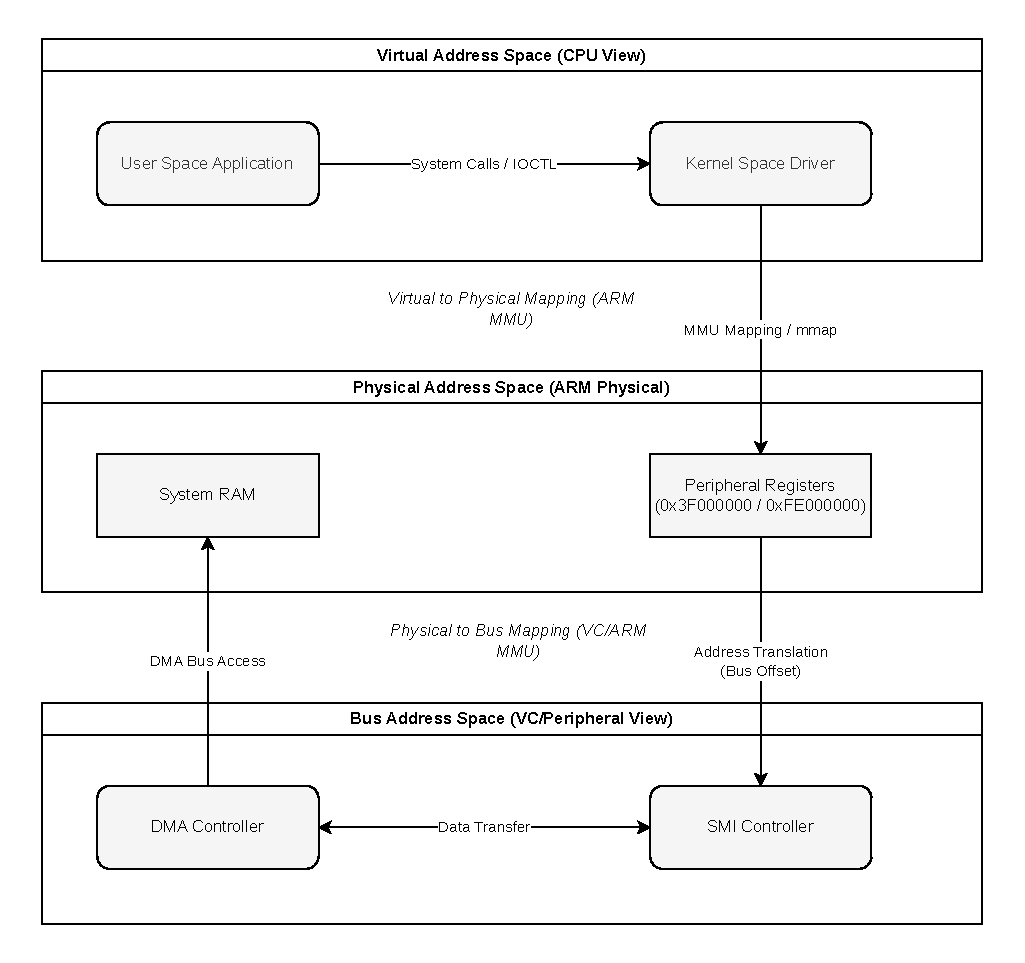
\includegraphics[width=1\textwidth]{img/bcm-address-translation.pdf}
\end{cmpfigure}

\begin{cmpfigure}[htb]{SMI Architecture Block Diagram~\cite{zotero-item-12}\label{smi_block_diagram}}
    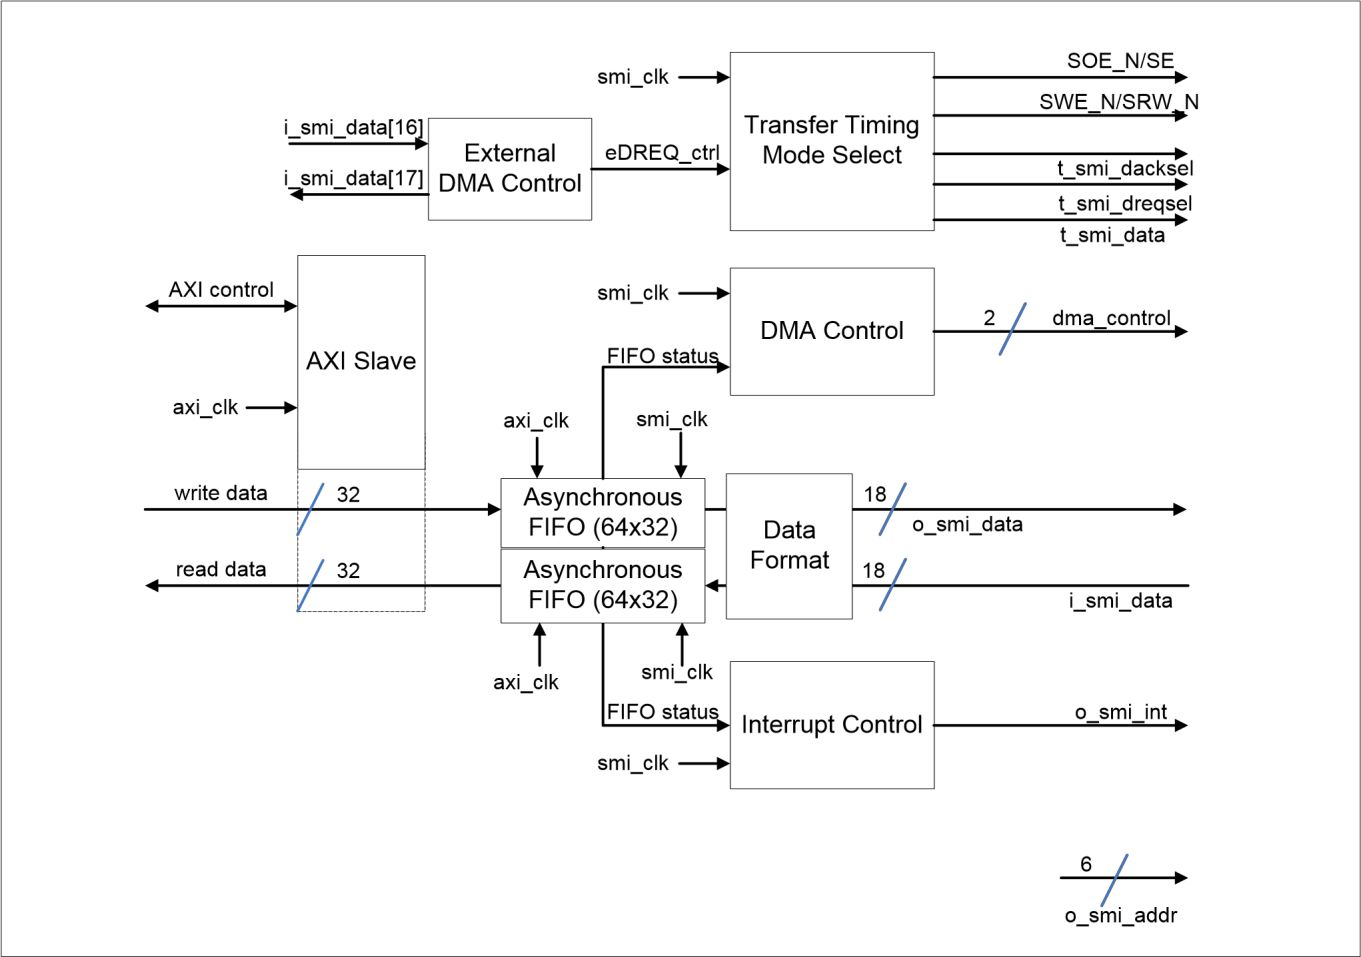
\includegraphics[width=1\textwidth]{img/smi-block-diagram.jpg}
\end{cmpfigure}

\begin{cmpfigure}[htb]{System Architecture\label{system_architecture}}
    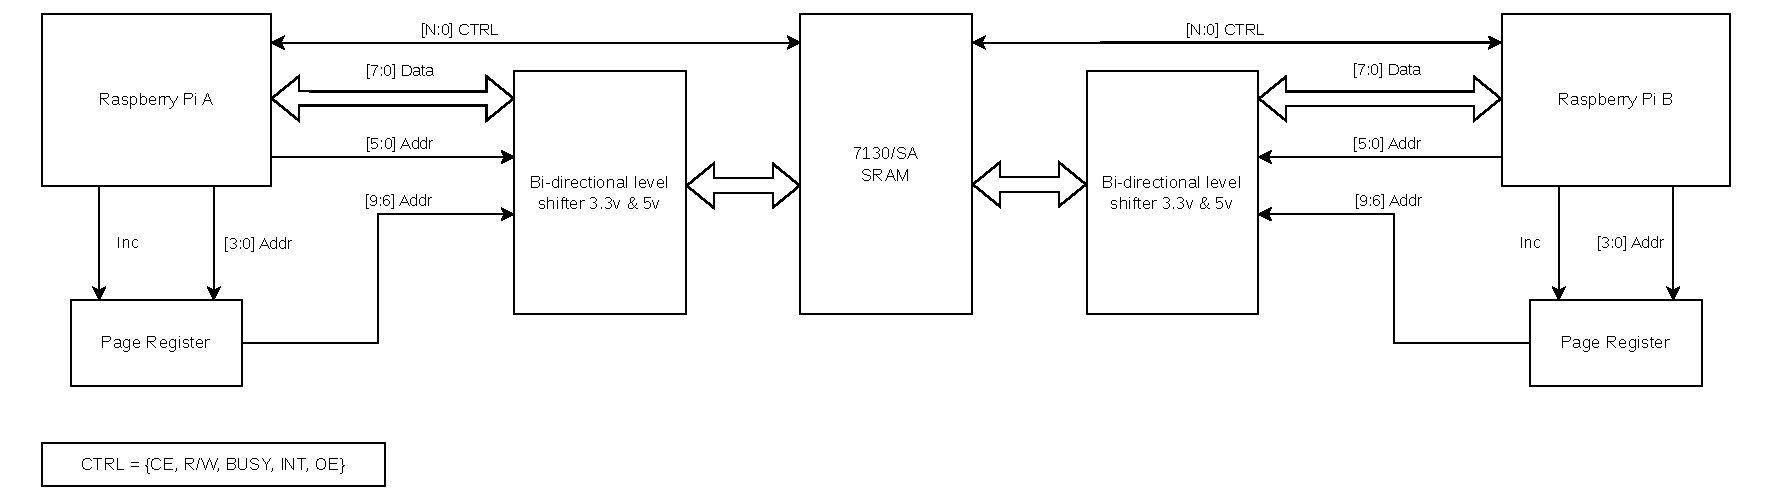
\includegraphics[width=1\textwidth]{img/rpismi-arch.pdf}
\end{cmpfigure}

\begin{cmpfigure}[htb]{Software Architecture\label{software_architecture}}
    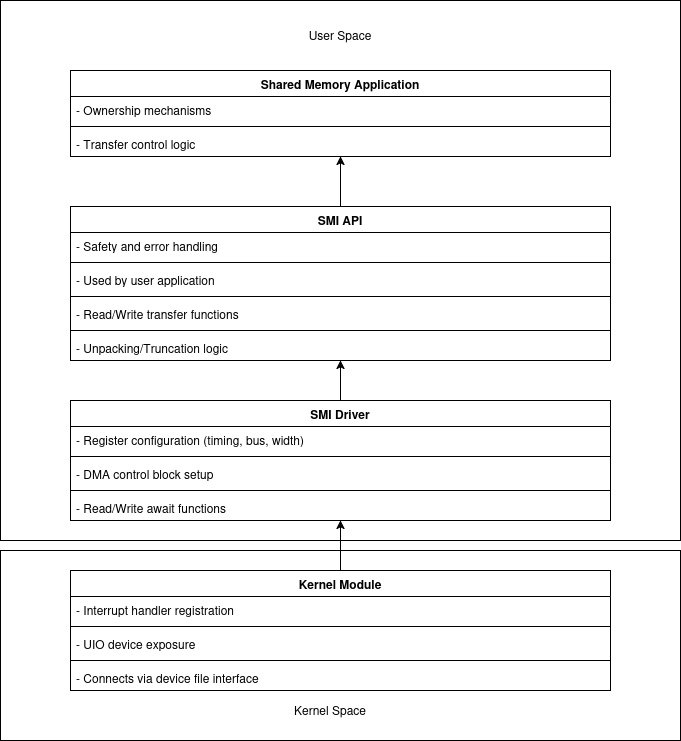
\includegraphics[width=1\textwidth]{img/rpismi_softarch.png}
\end{cmpfigure}

\begin{cmpfigure}[htb]{Read Await Function Flow Diagram\label{read_await}}
    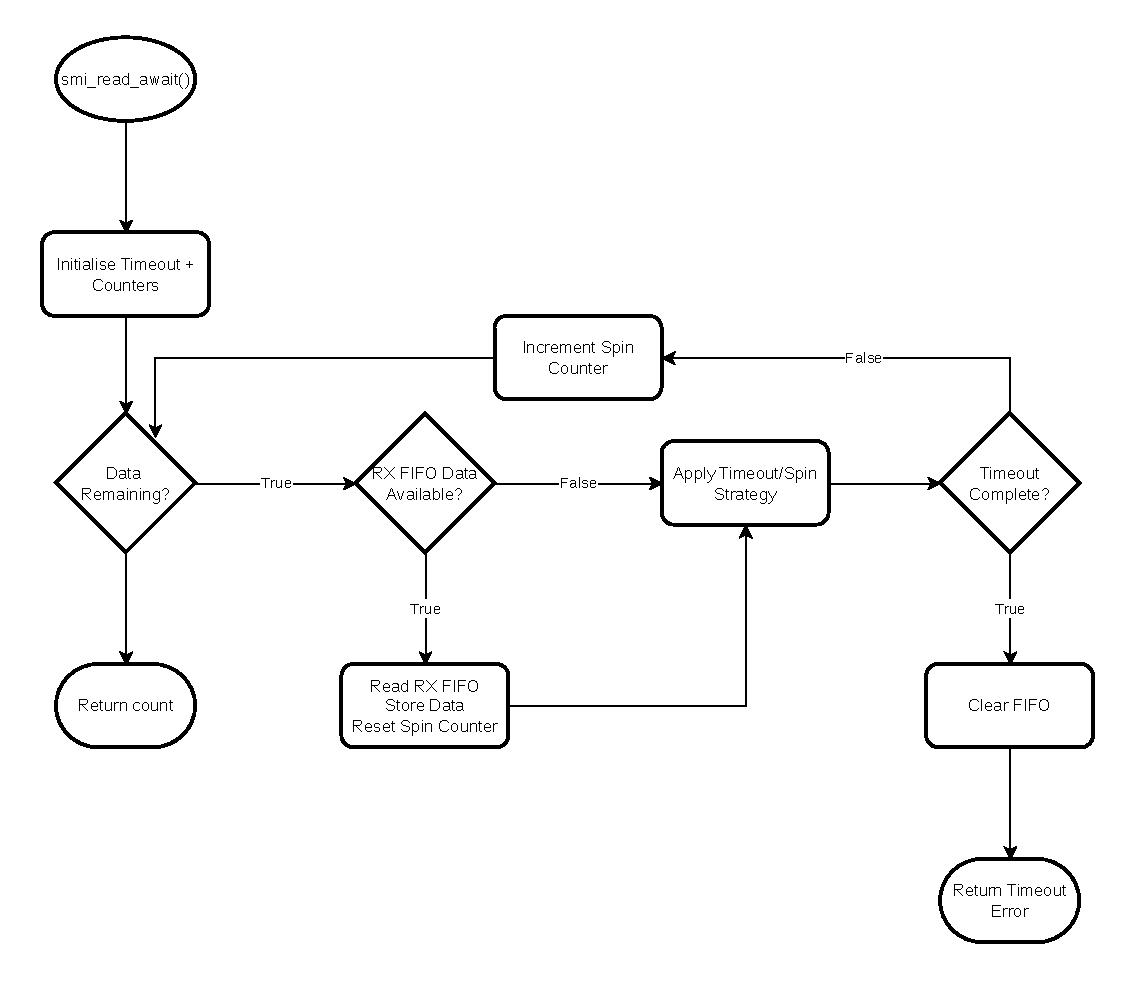
\includegraphics[width=1\textwidth]{img/rpismi_read_await.pdf}
\end{cmpfigure}

\begin{cmpfigure}[htb]{DMA Transfer Data Flow Diagram\label{dma_flow}}
    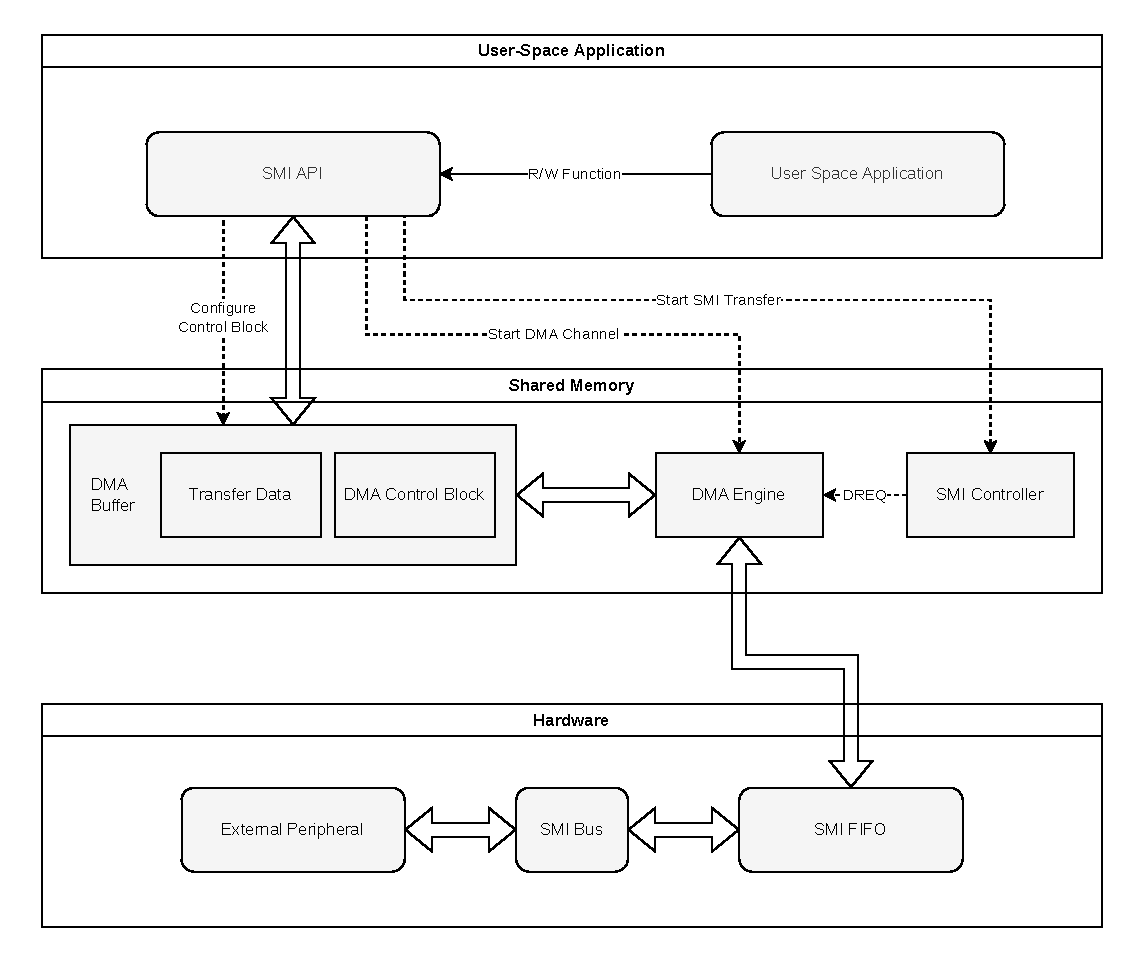
\includegraphics[width=1\textwidth]{img/rpismi-dma-transfer.pdf}
\end{cmpfigure}

\begin{cmpfigure}[htb]{Timeout Strategy Tiers\label{timeout_strat}}
    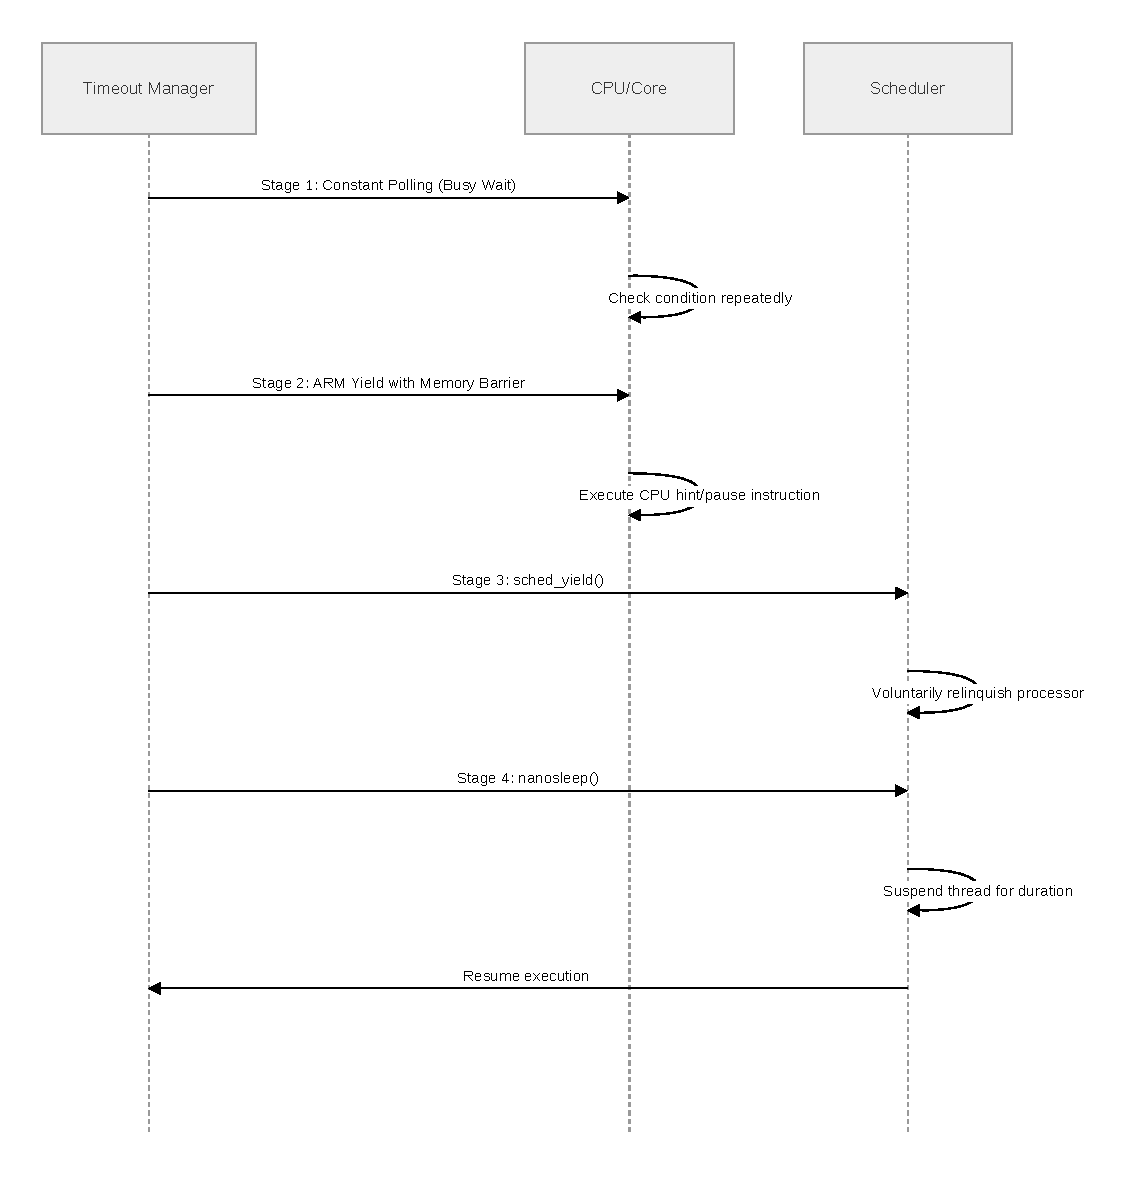
\includegraphics[width=1\textwidth]{img/rpismi_timeout_strategy.pdf}
\end{cmpfigure}

\begin{cmpfigure}[htb]{8-bit Interface Packing~\cite{zotero-item-12}\label{8_bit_pack}}
    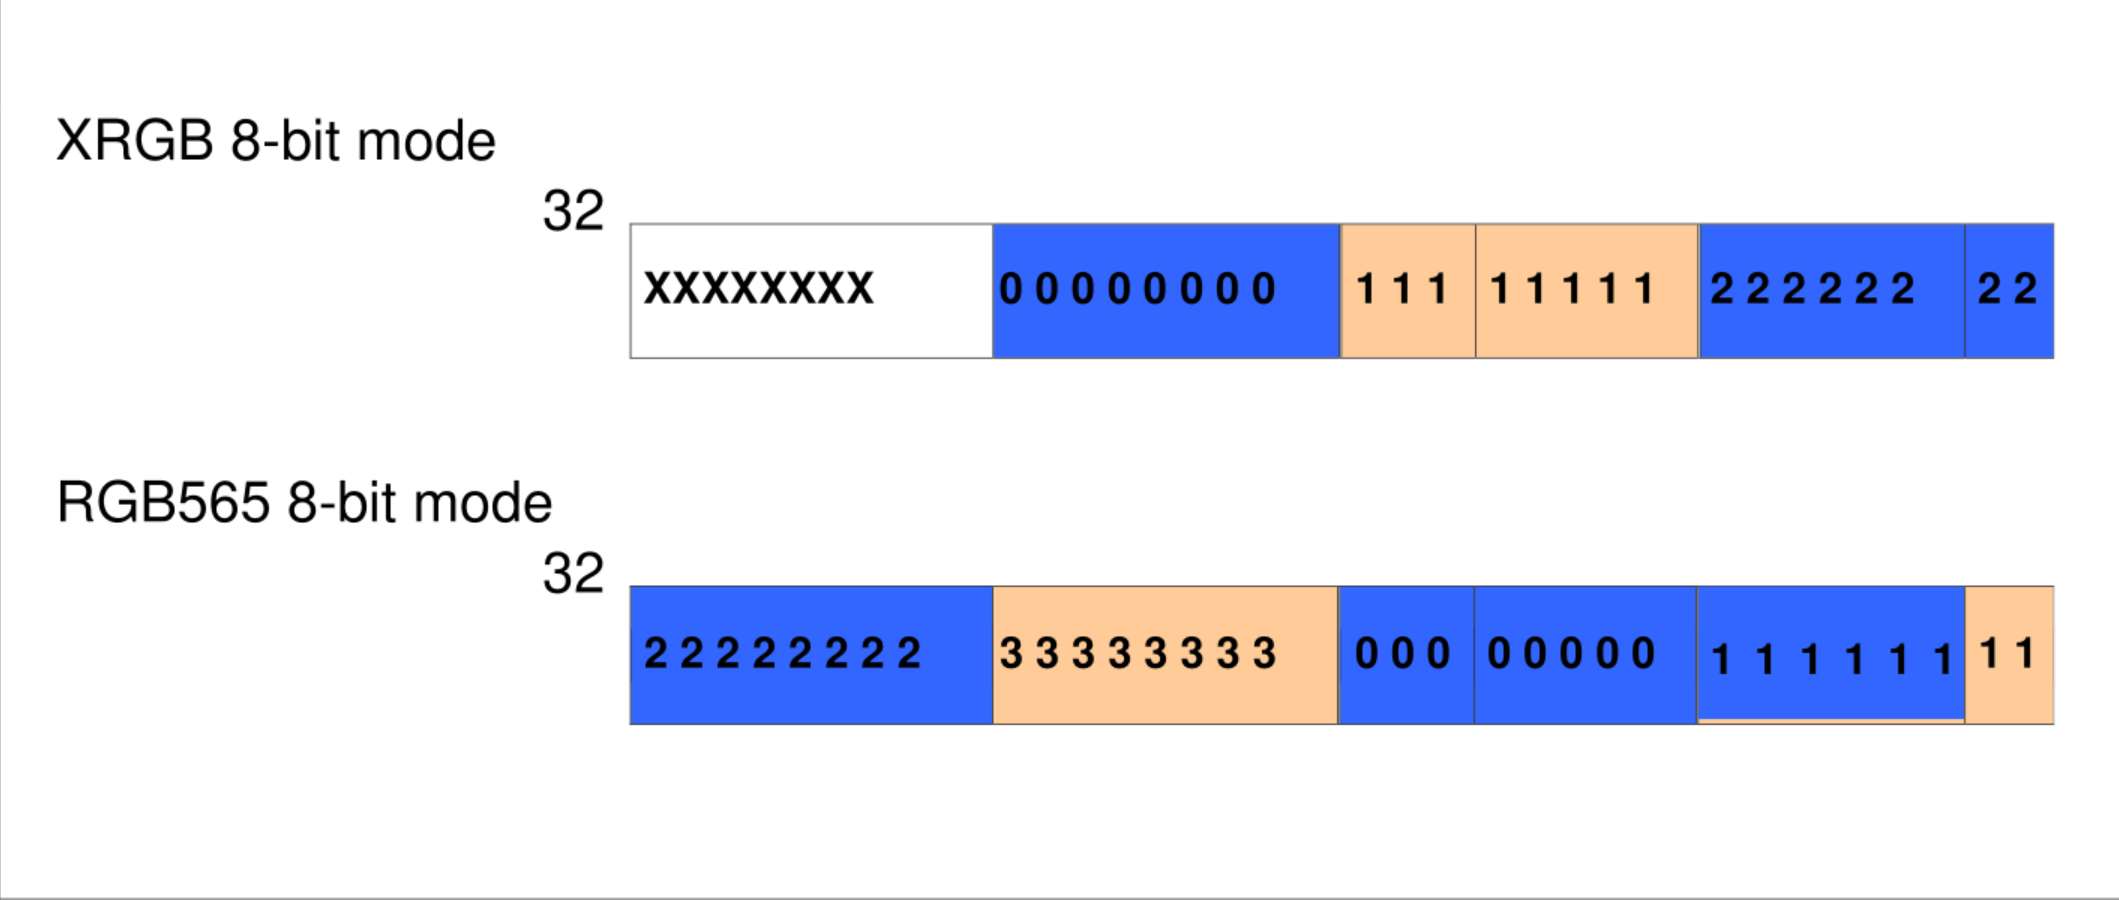
\includegraphics[width=1\textwidth]{img/8-bit-pack.png}
\end{cmpfigure}

\begin{cmpfigure}[htb]{Raspberry Pi 3B+ SMI No Packing Throughput MT/s vs Block Size (O3, 32-bit OS)~\label{3b_throughput_mts_nopacked}}
    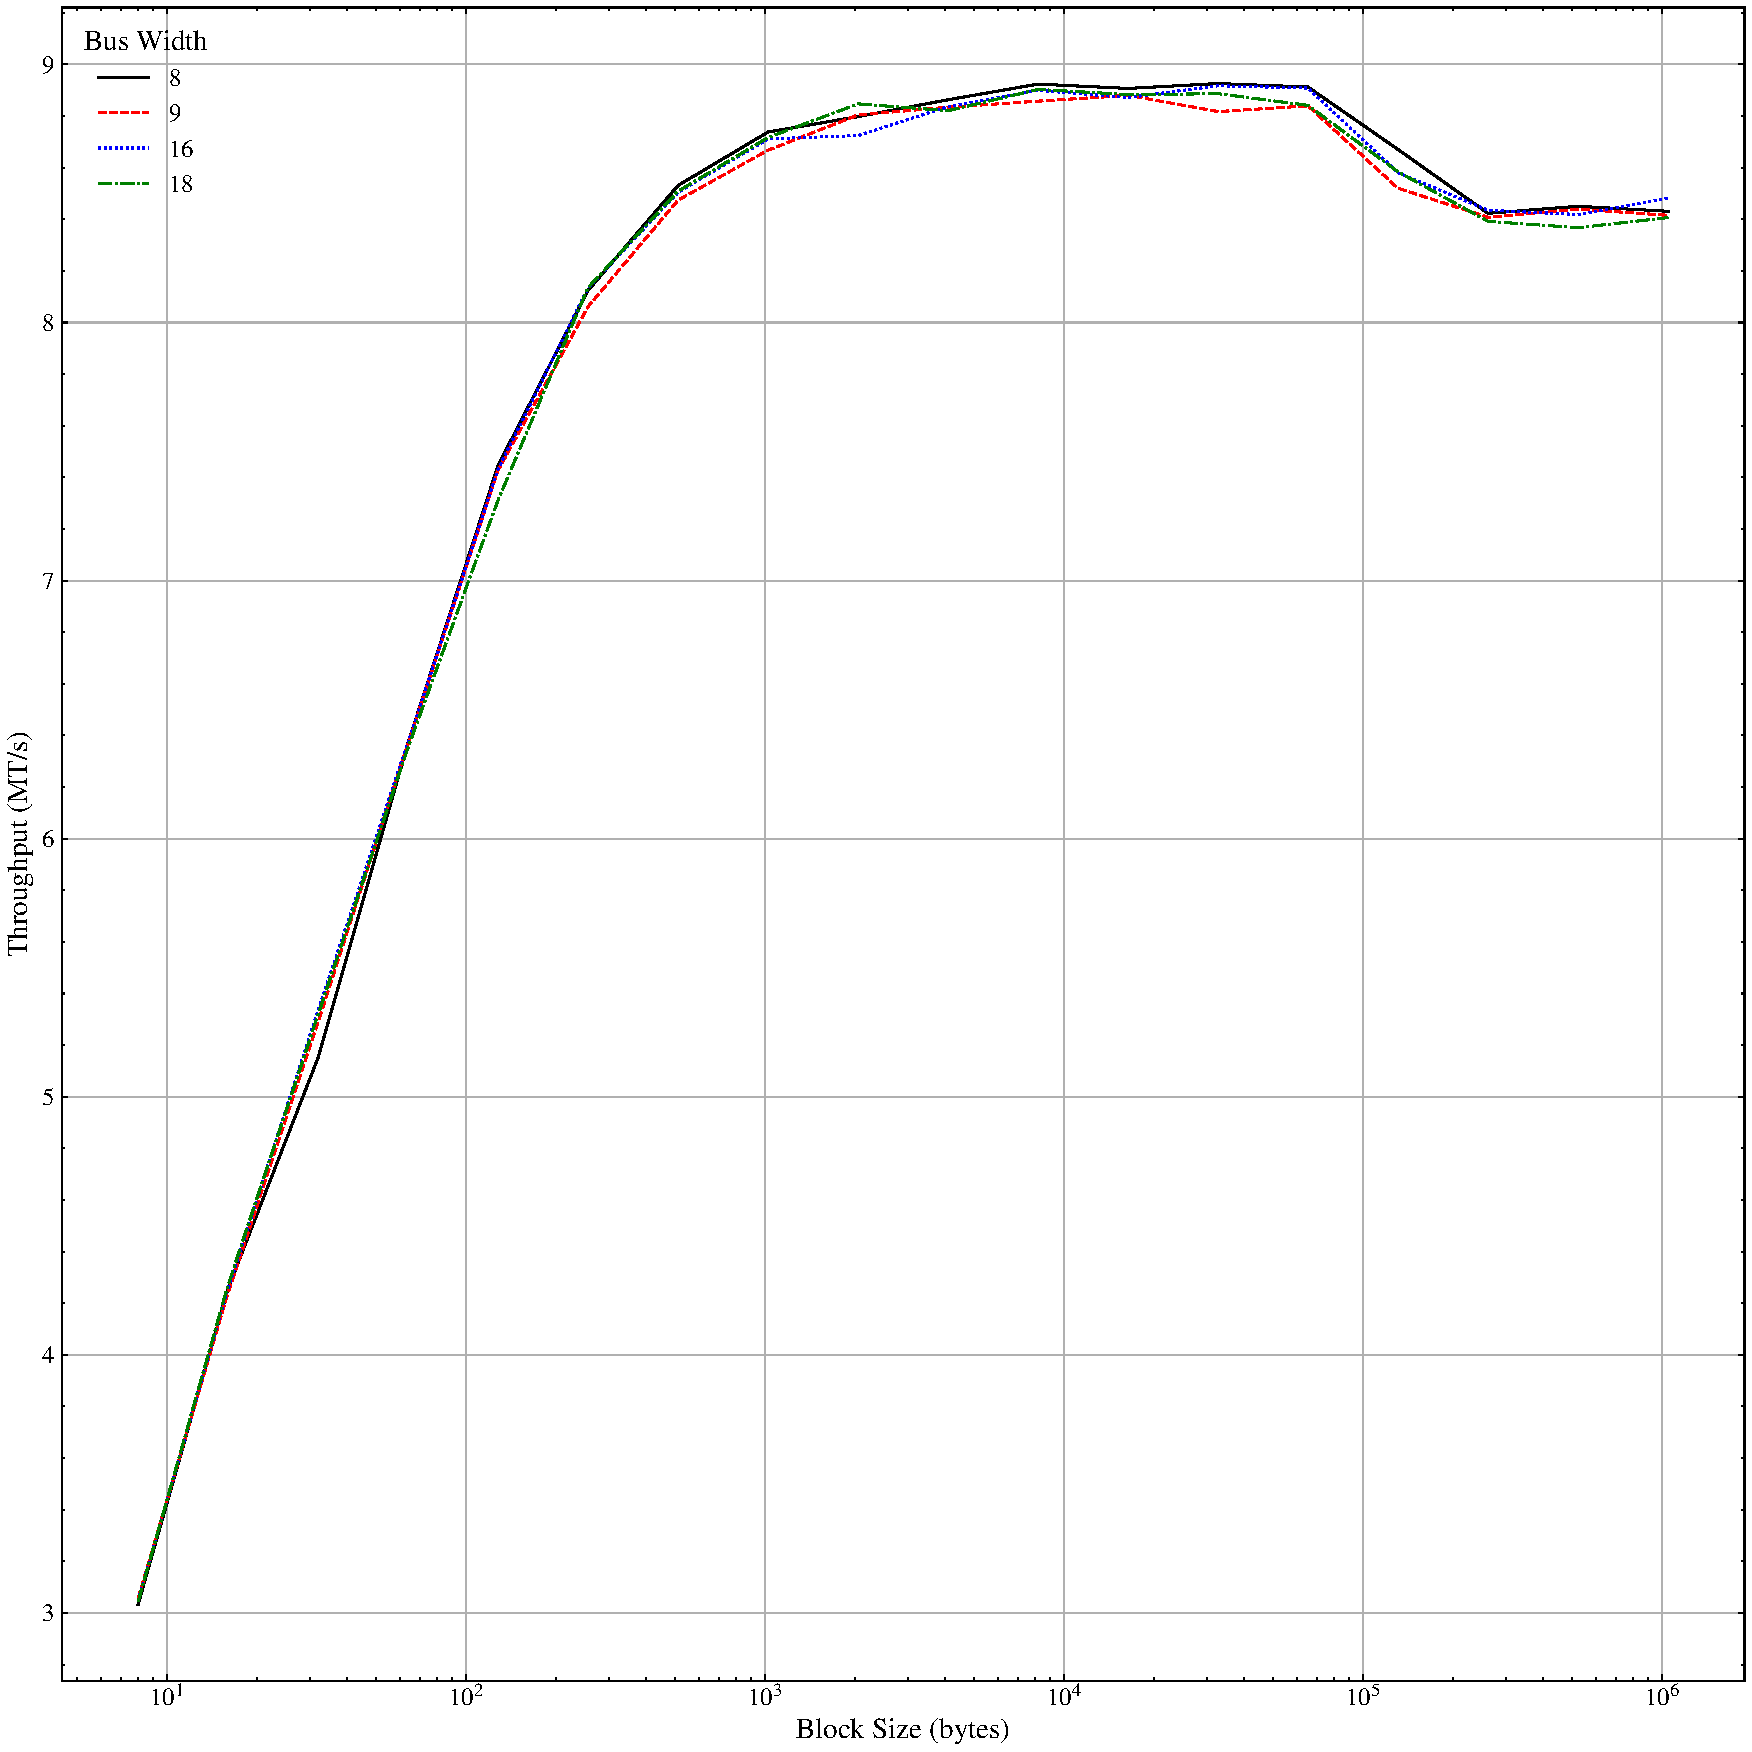
\includegraphics[width=1\textwidth]{img/rpi3b-smi-unpacked-mts.pdf}
\end{cmpfigure}

\begin{cmpfigure}[htb]{Raspberry Pi 3B+ SMI No Packing Throughput MB/s vs Block Size (O3, 32-bit OS)~\label{3b_throughput_mbs_nopacked}}
    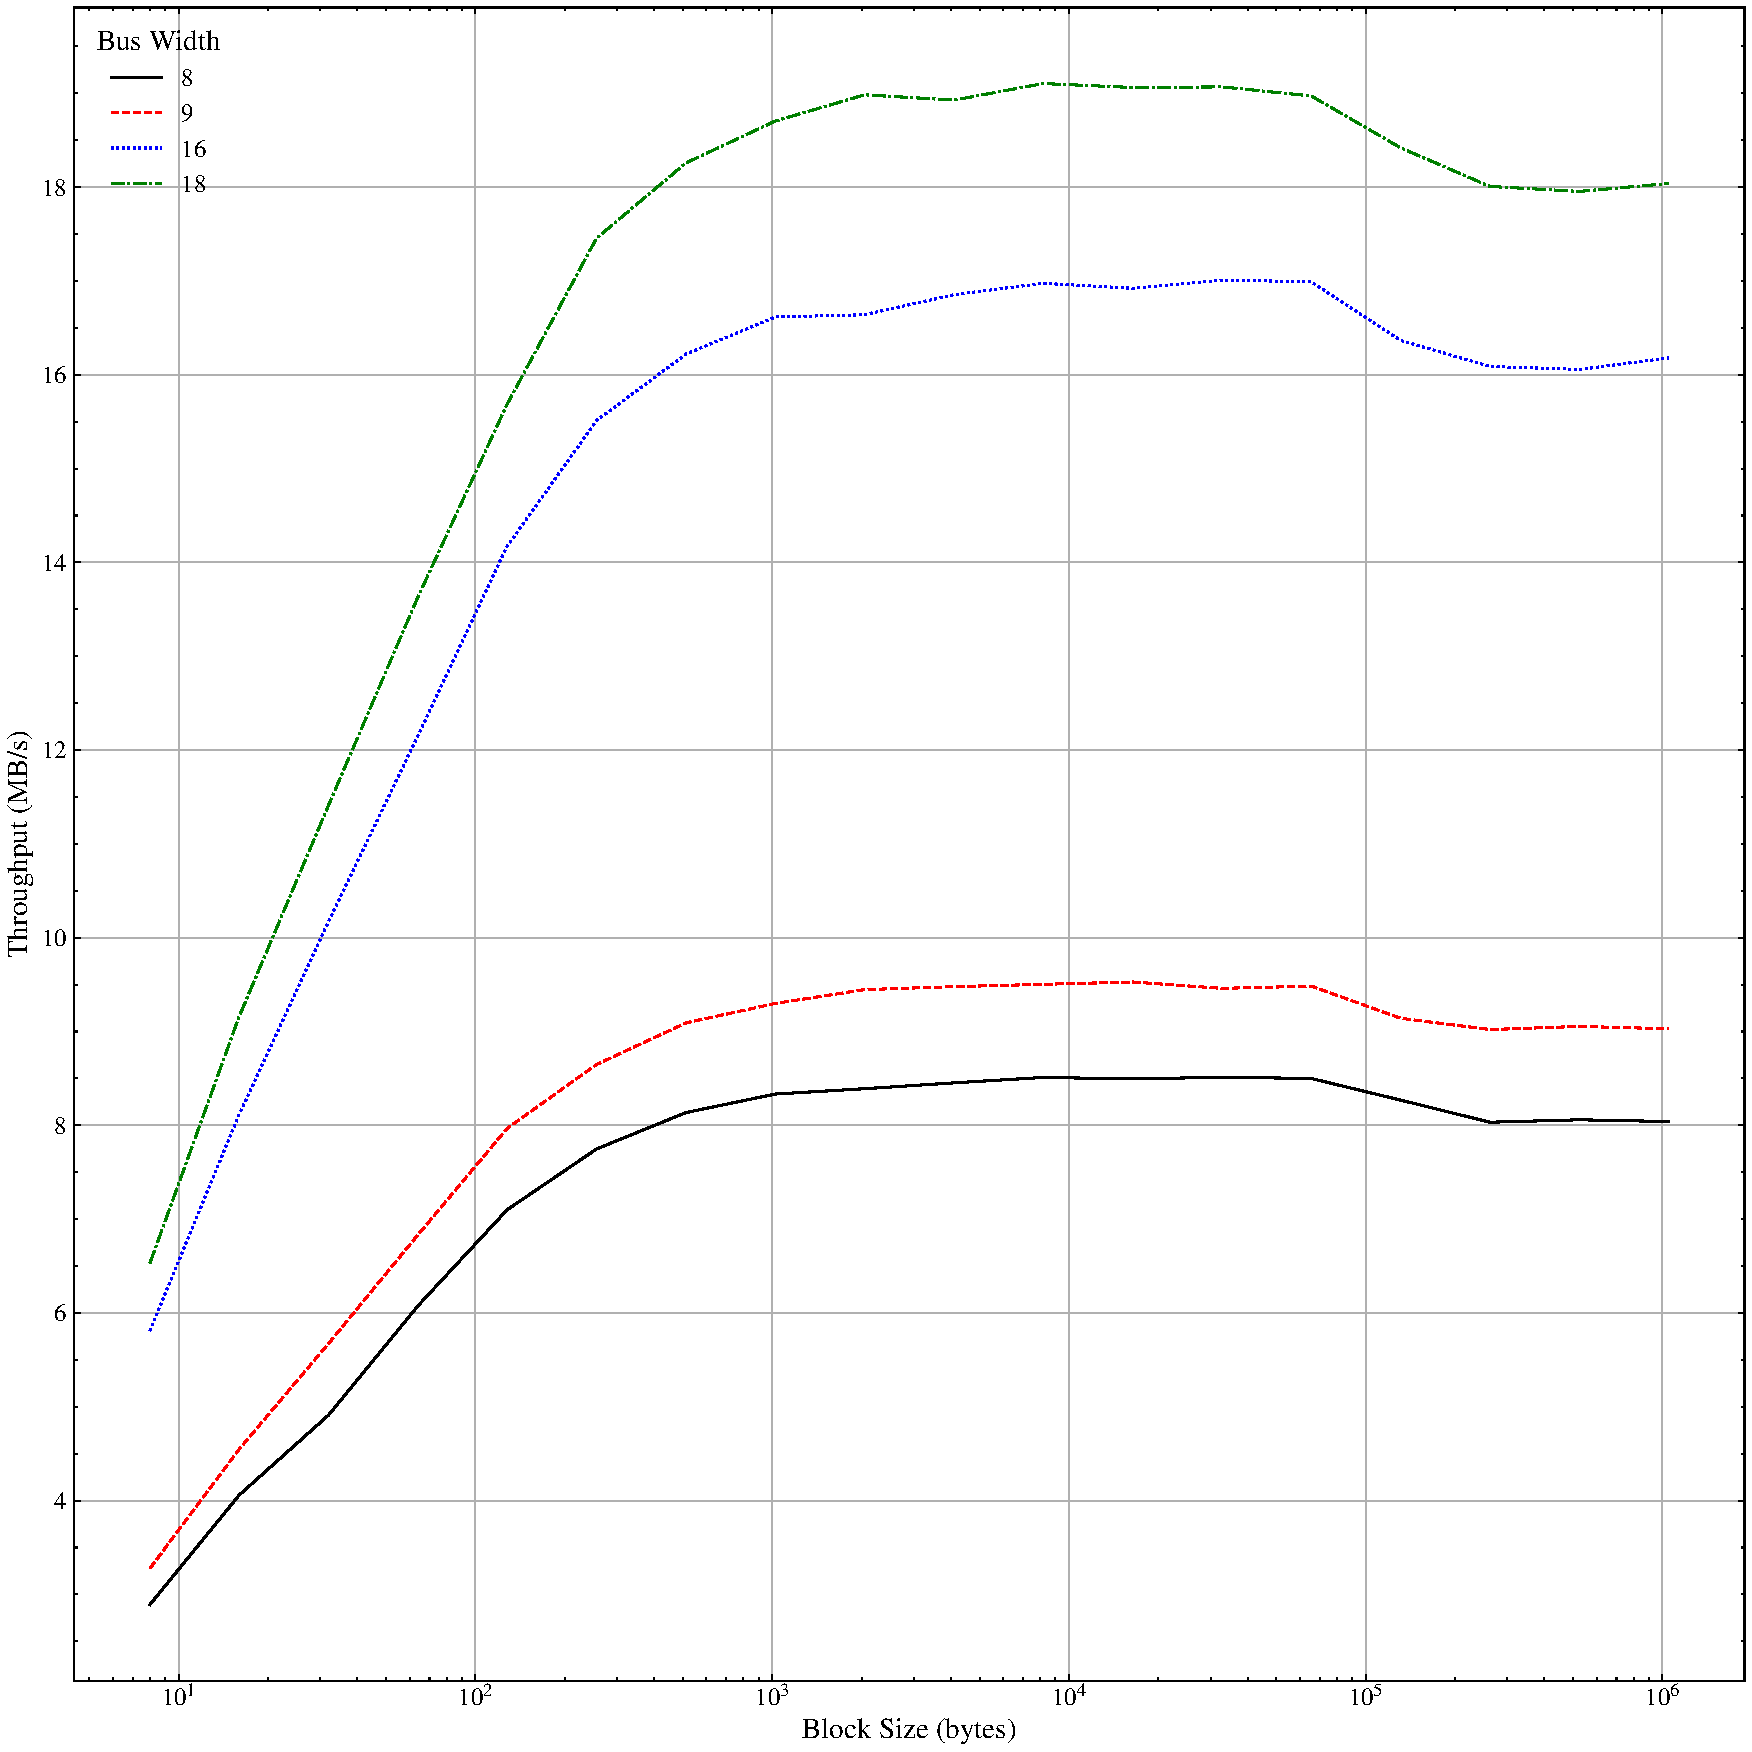
\includegraphics[width=1\textwidth]{img/rpi3b-smi-unpacked-mbs.pdf}
\end{cmpfigure}

\begin{cmpfigure}[htb]{Raspberry Pi 3B+ SMI No Packing Duration vs Block Size (O3, 32-bit OS)~\label{3b_throughput_duration_nopacked}}
    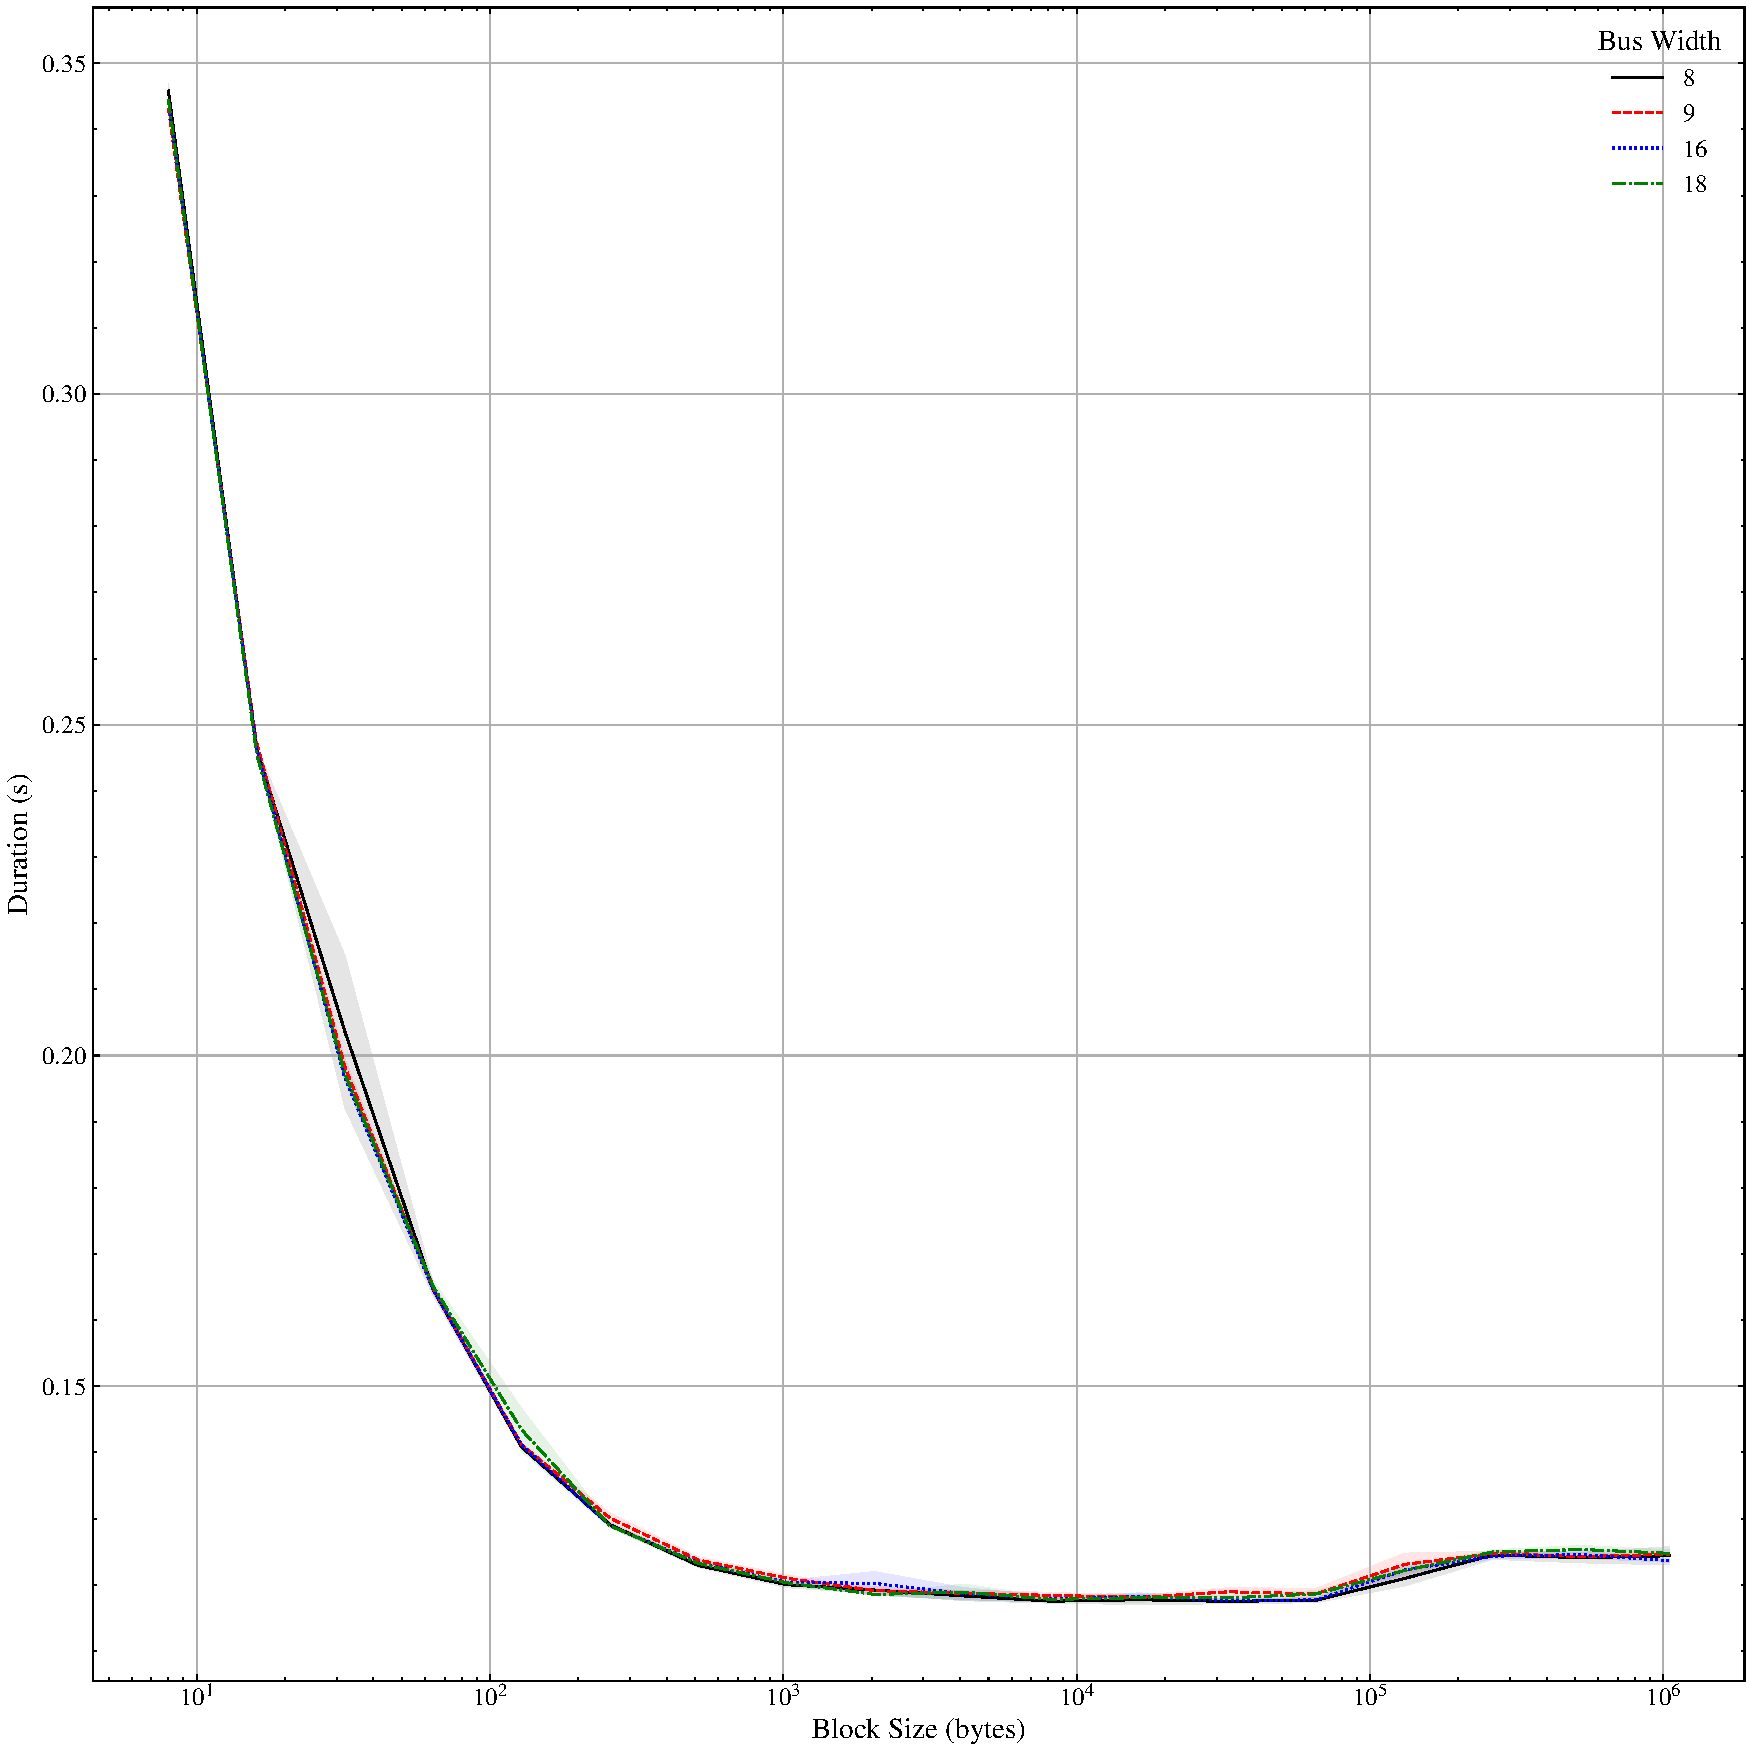
\includegraphics[width=1\textwidth]{img/rpi3b-smi-unpacked-duration.pdf}
\end{cmpfigure}

\begin{cmpfigure}[htb]{Raspberry Pi 3B+ SMI Throughput MT/s vs Block Size (O3, 32-bit OS)~\label{3b_throughput_mts}}
    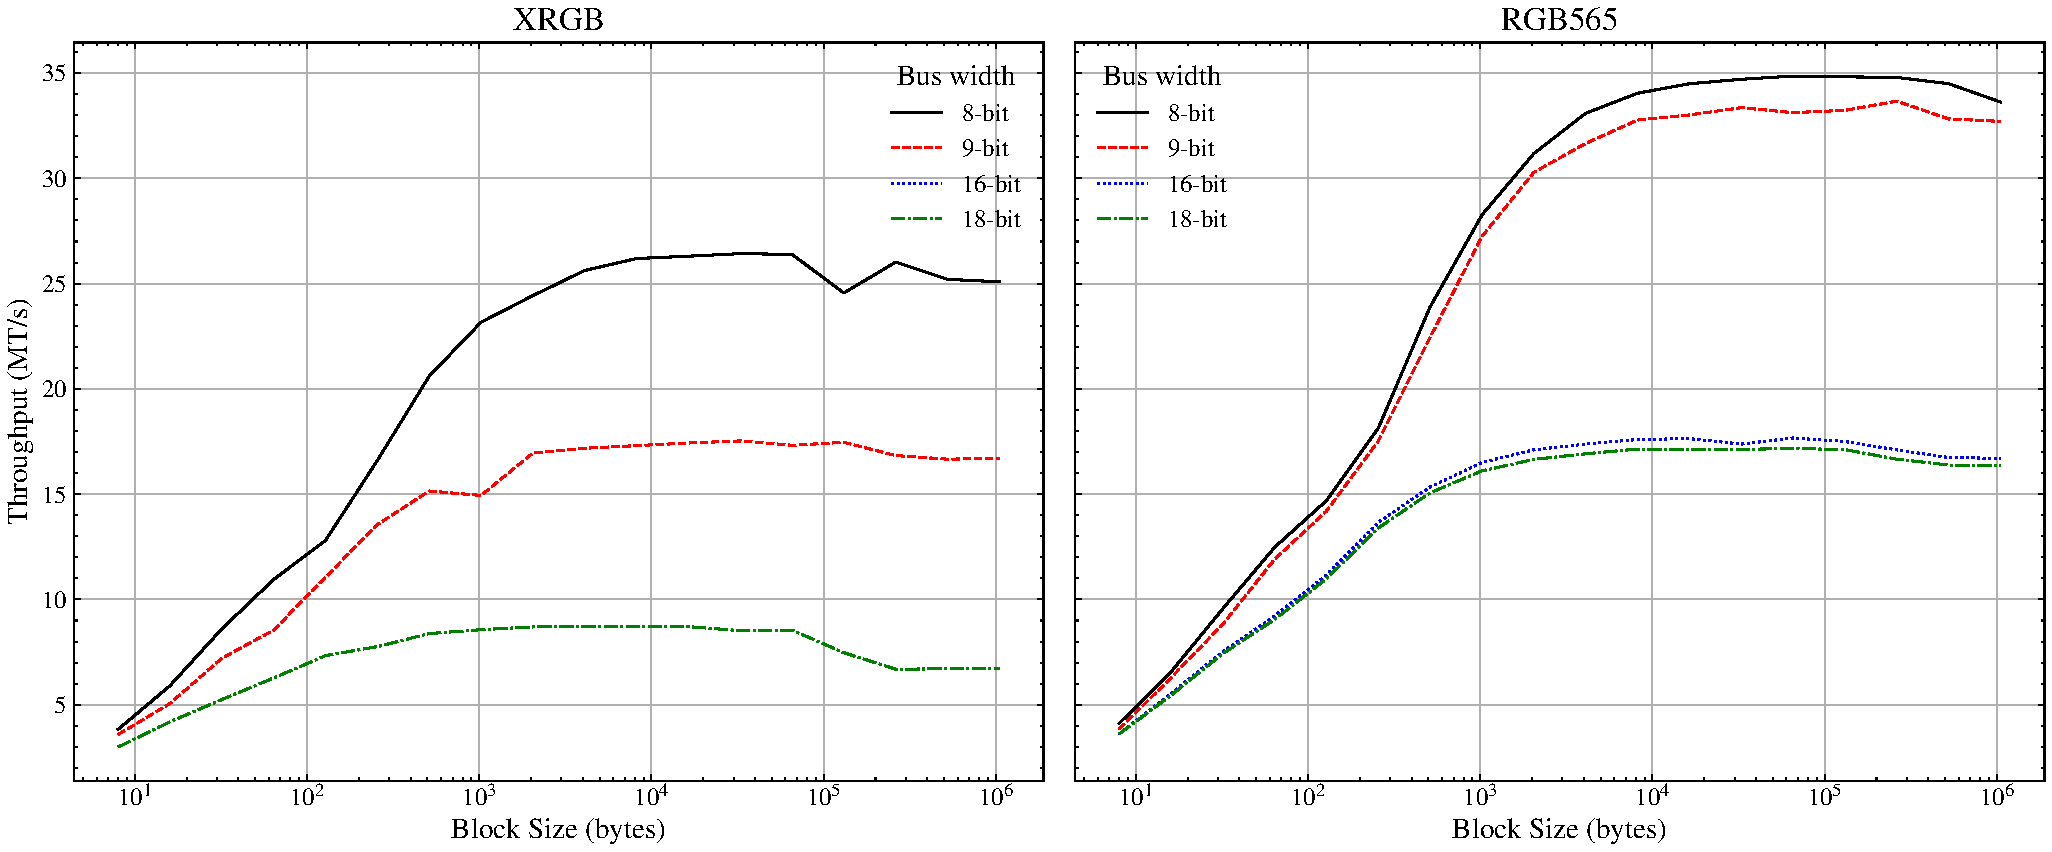
\includegraphics[width=1\textwidth]{img/rpi3b-smi-throughput-mts.pdf}
\end{cmpfigure}

\begin{cmpfigure}[htb]{Raspberry Pi 3B+ SMI Throughput MB/s vs Block Size (O3, 32-bit OS)~\label{3b_throughput_mbs}}
    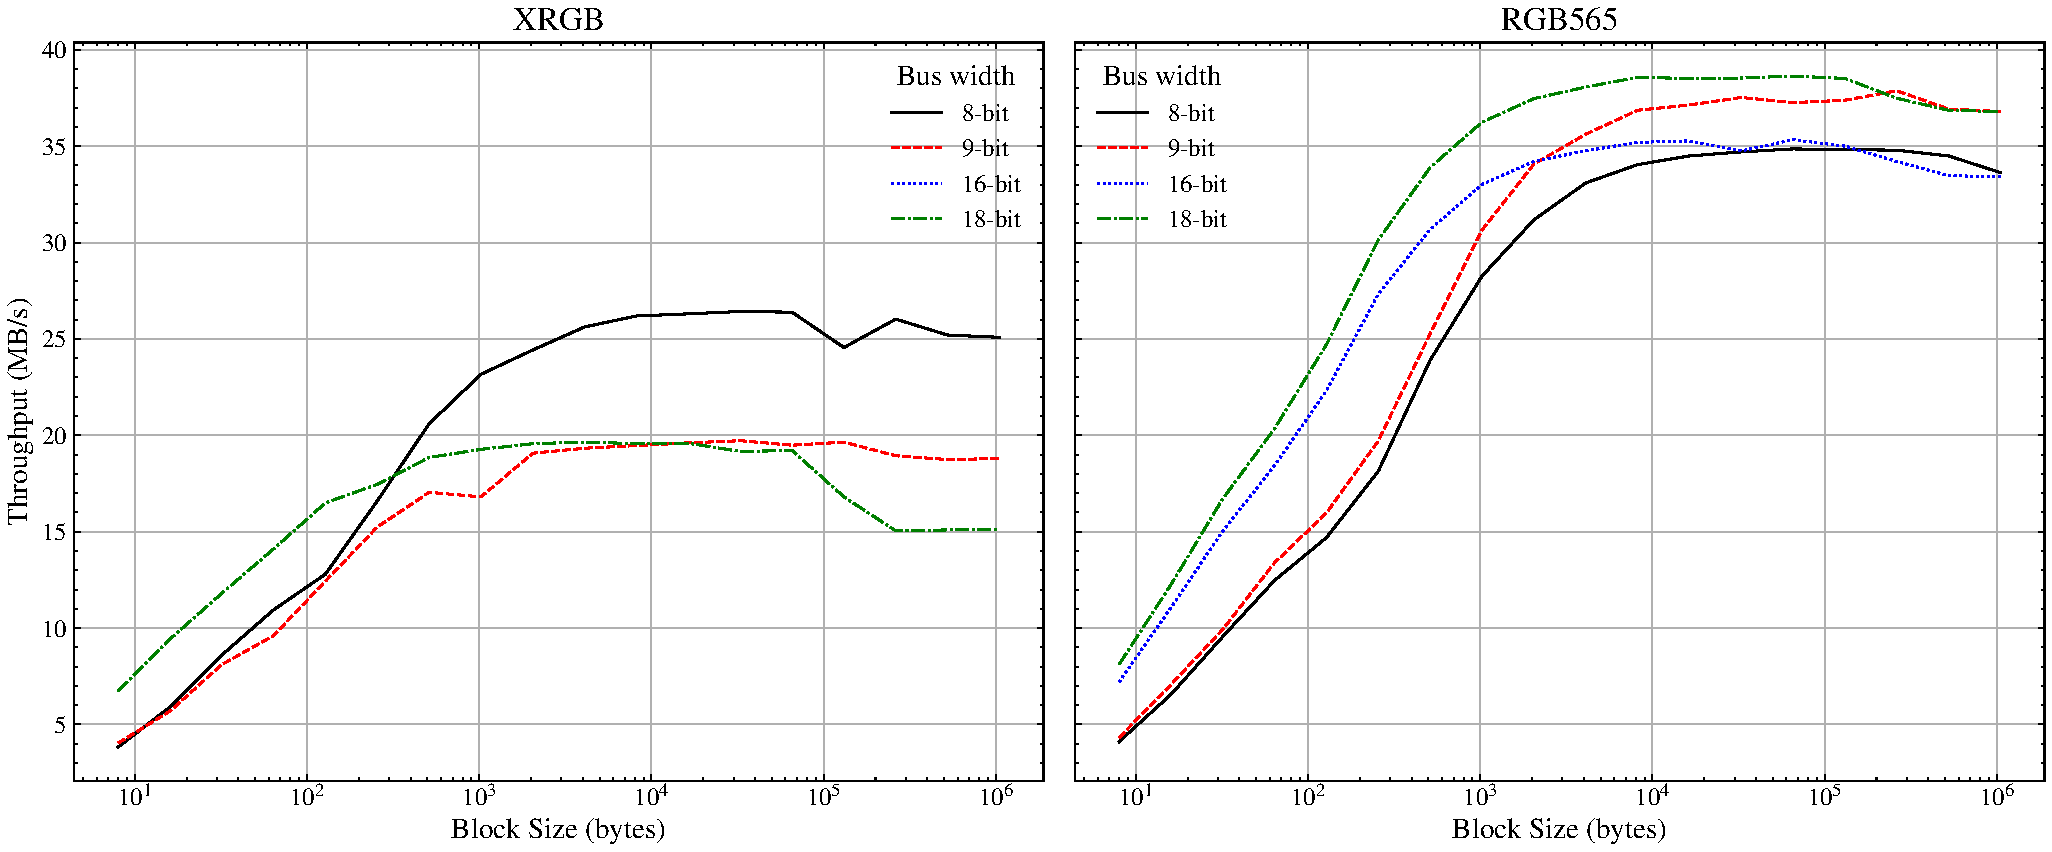
\includegraphics[width=1\textwidth]{img/rpi3b-smi-throughput-mbs.pdf}
\end{cmpfigure}

\begin{cmpfigure}[htb]{Raspberry Pi 3B+ SMI Duration vs Block Size (O3, 32-bit OS)~\label{3b_throughput_duration}}
    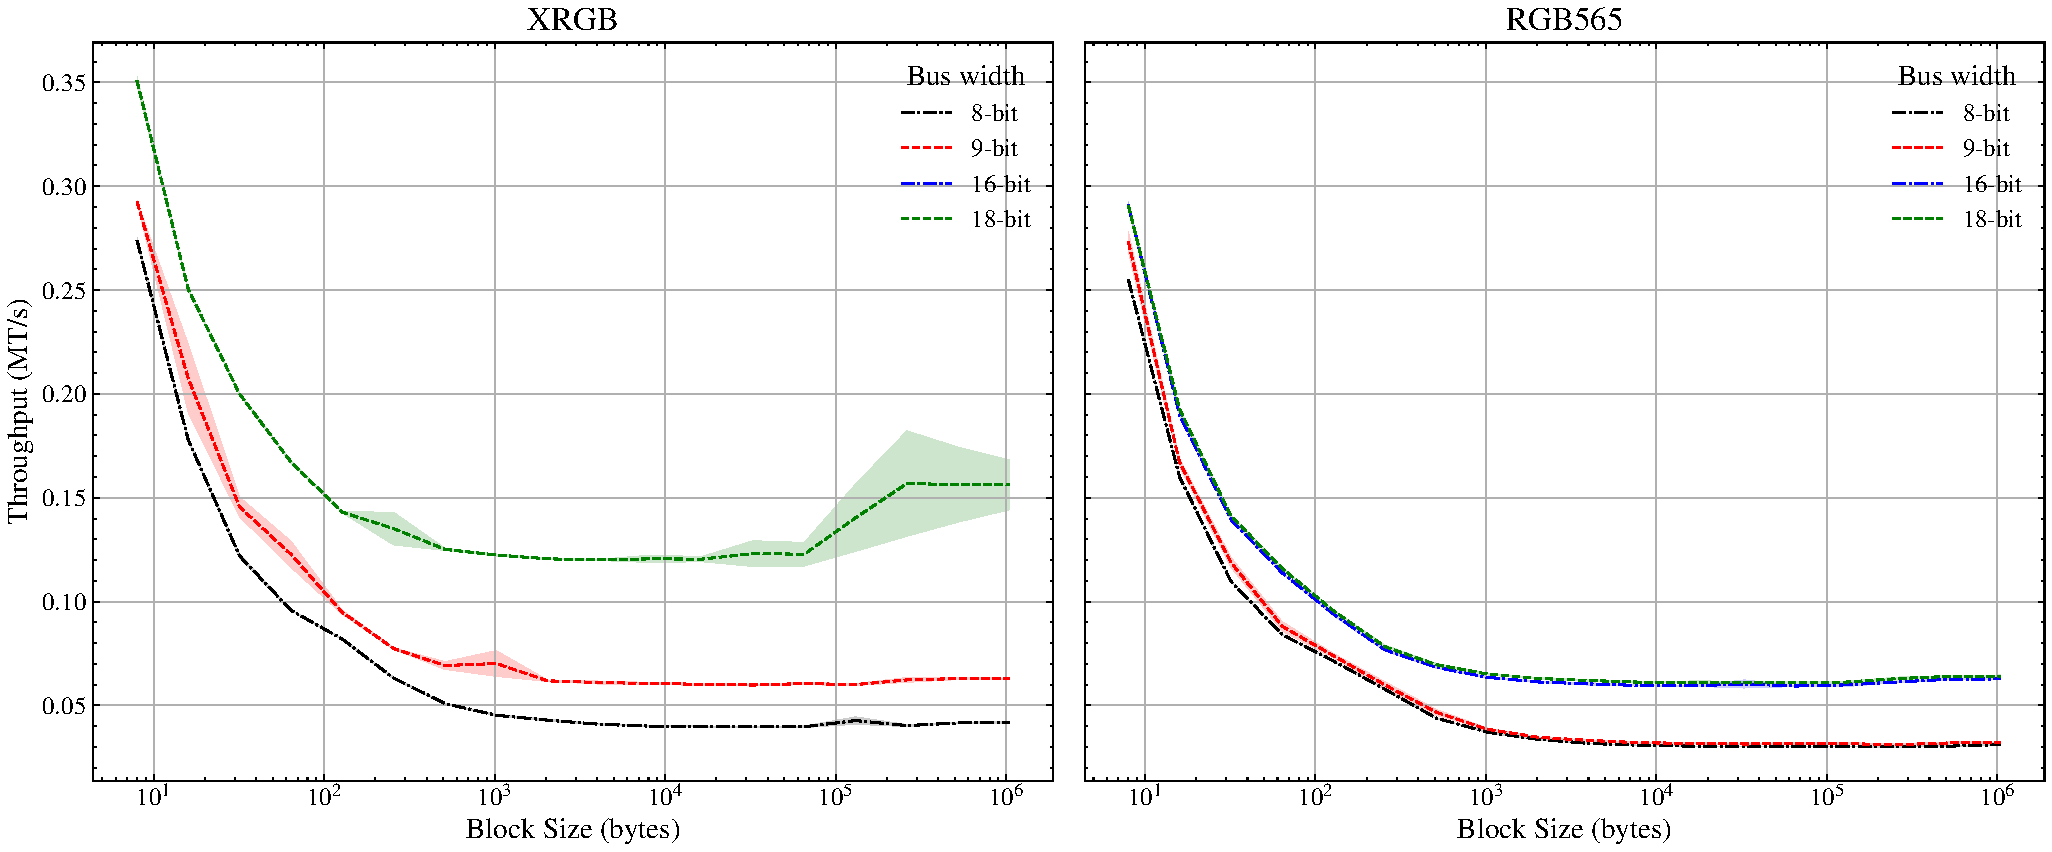
\includegraphics[width=1\textwidth]{img/rpi3b-smi-duration.pdf}
\end{cmpfigure}

\begin{cmpfigure}[htb]{Raspberry Pi 3B+ SMI Throughput MT/s vs Block Size (O3, 64-bit OS)~\label{3b_64_throughput_mts}}
    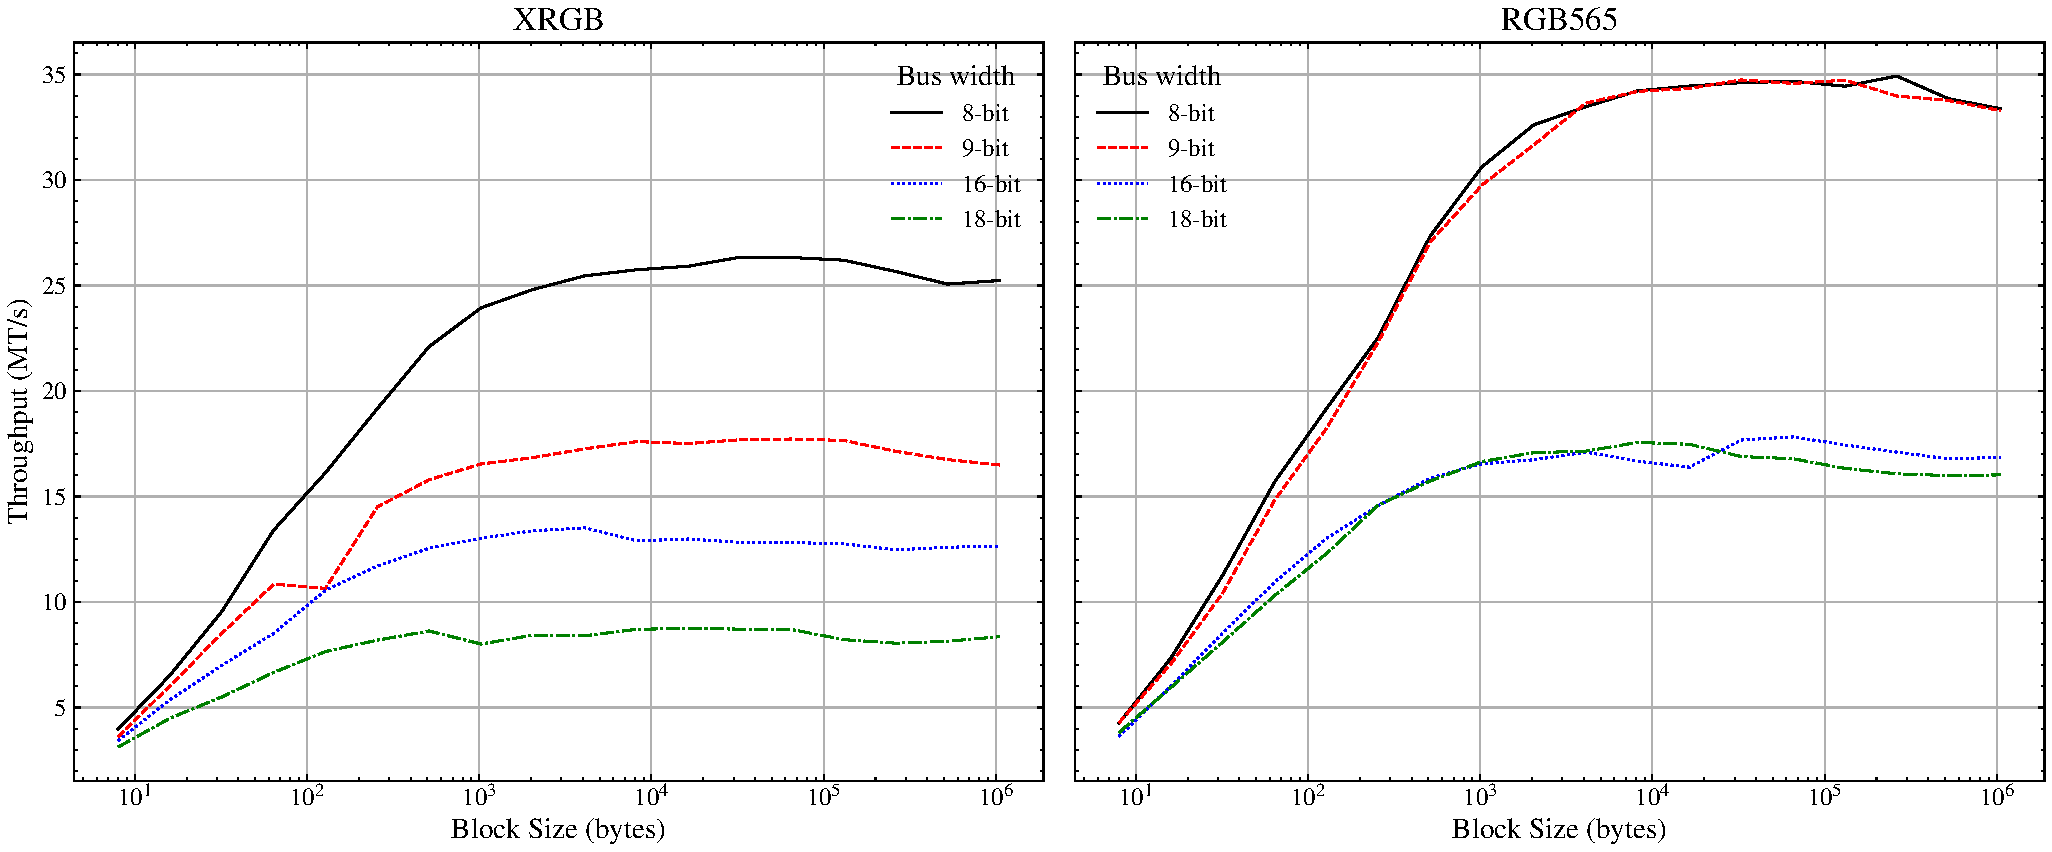
\includegraphics[width=1\textwidth]{img/rpi3b-64-smi-throughput-mts.pdf}
\end{cmpfigure}

\begin{cmpfigure}[htb]{Raspberry Pi 3B+ SMI Throughput MB/s vs Block Size (O3, 64-bit OS)~\label{3b_64_throughput_mbs}}
    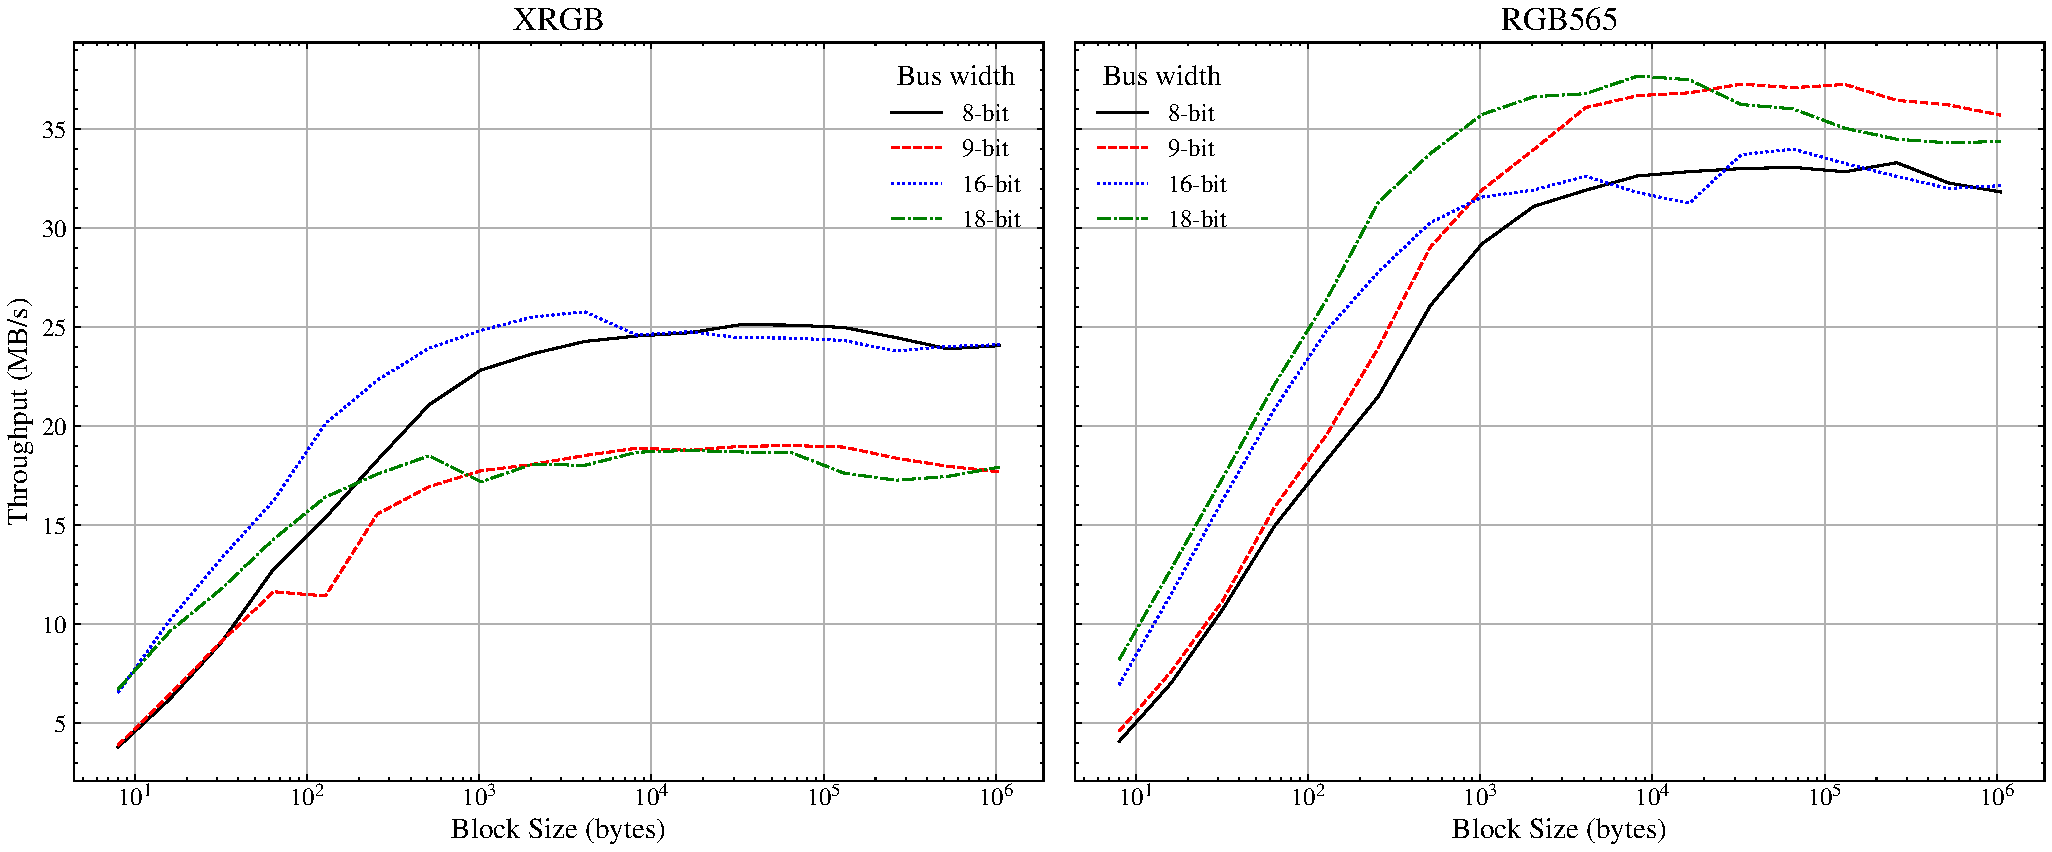
\includegraphics[width=1\textwidth]{img/rpi3b-64-smi-throughput-mbs.pdf}
\end{cmpfigure}

\begin{cmpfigure}[htb]{Raspberry Pi 3B+ SMI Duration vs Block Size (O3, 64-bit OS)~\label{3b_64_throughput_duration}}
    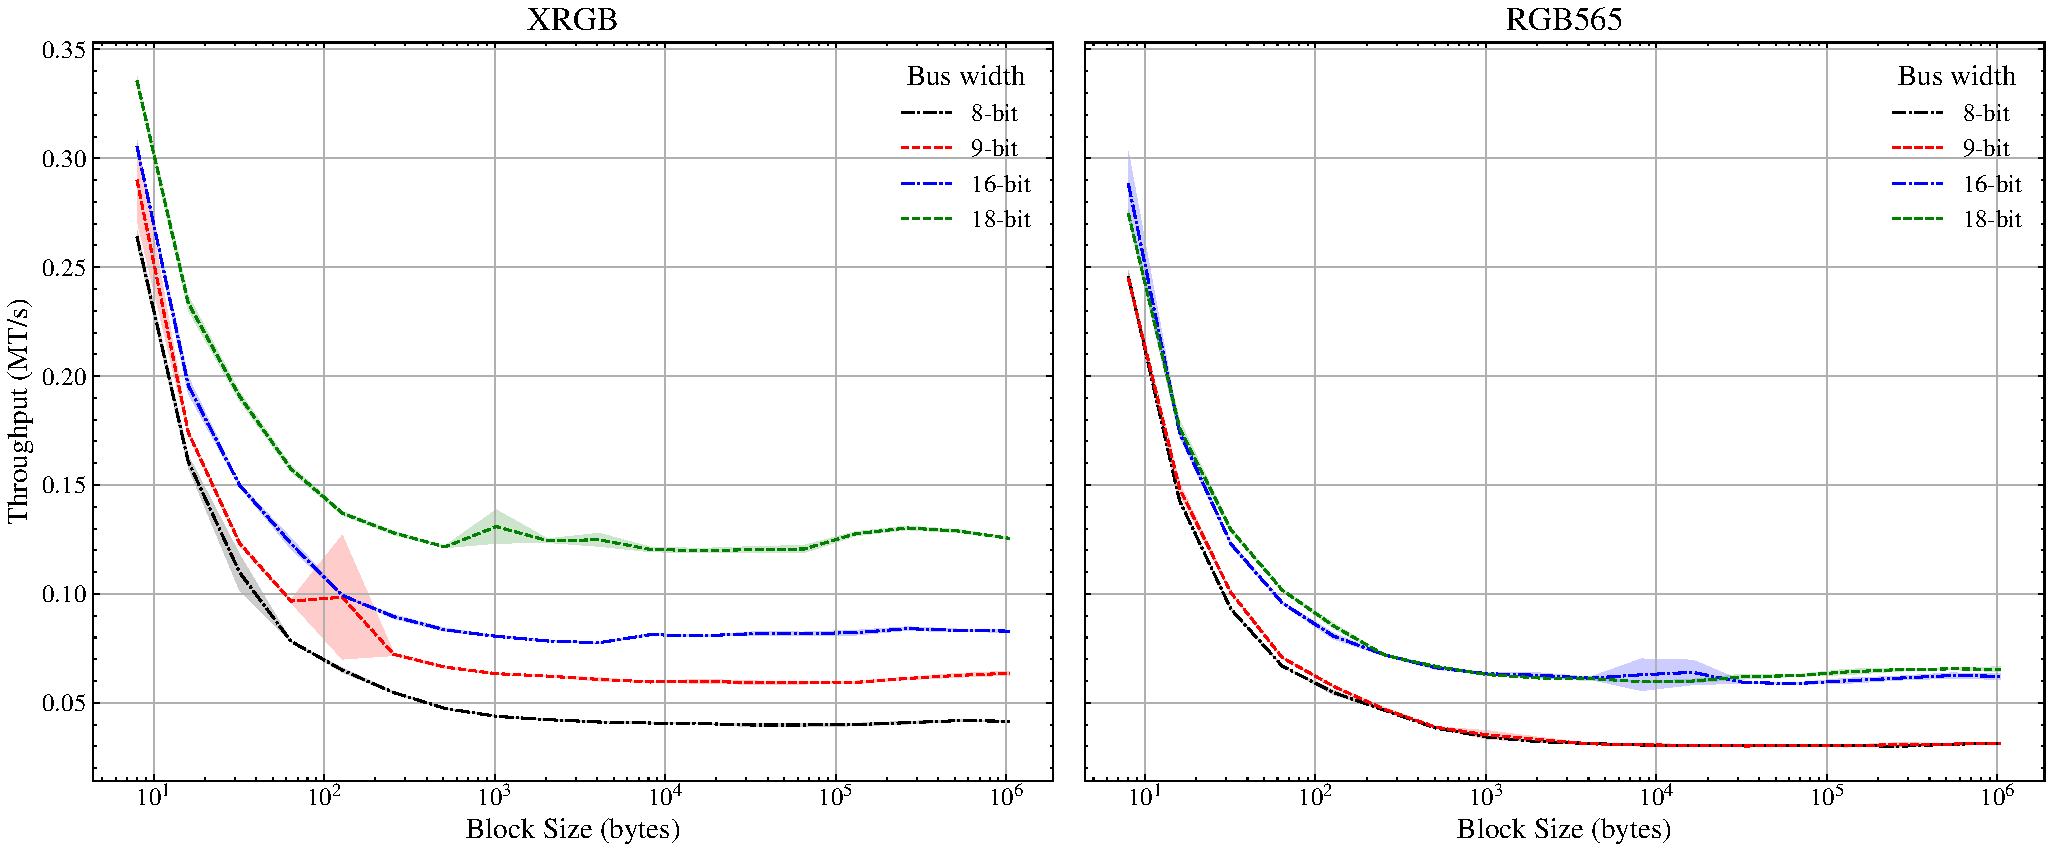
\includegraphics[width=1\textwidth]{img/rpi3b-64-smi-duration.pdf}
\end{cmpfigure}

\begin{cmpfigure}[htb]{Raspberry Pi 4 SMI Throughput MT/s vs Block Size (O3, 64-bit OS)~\label{4_throughput_mts}}
    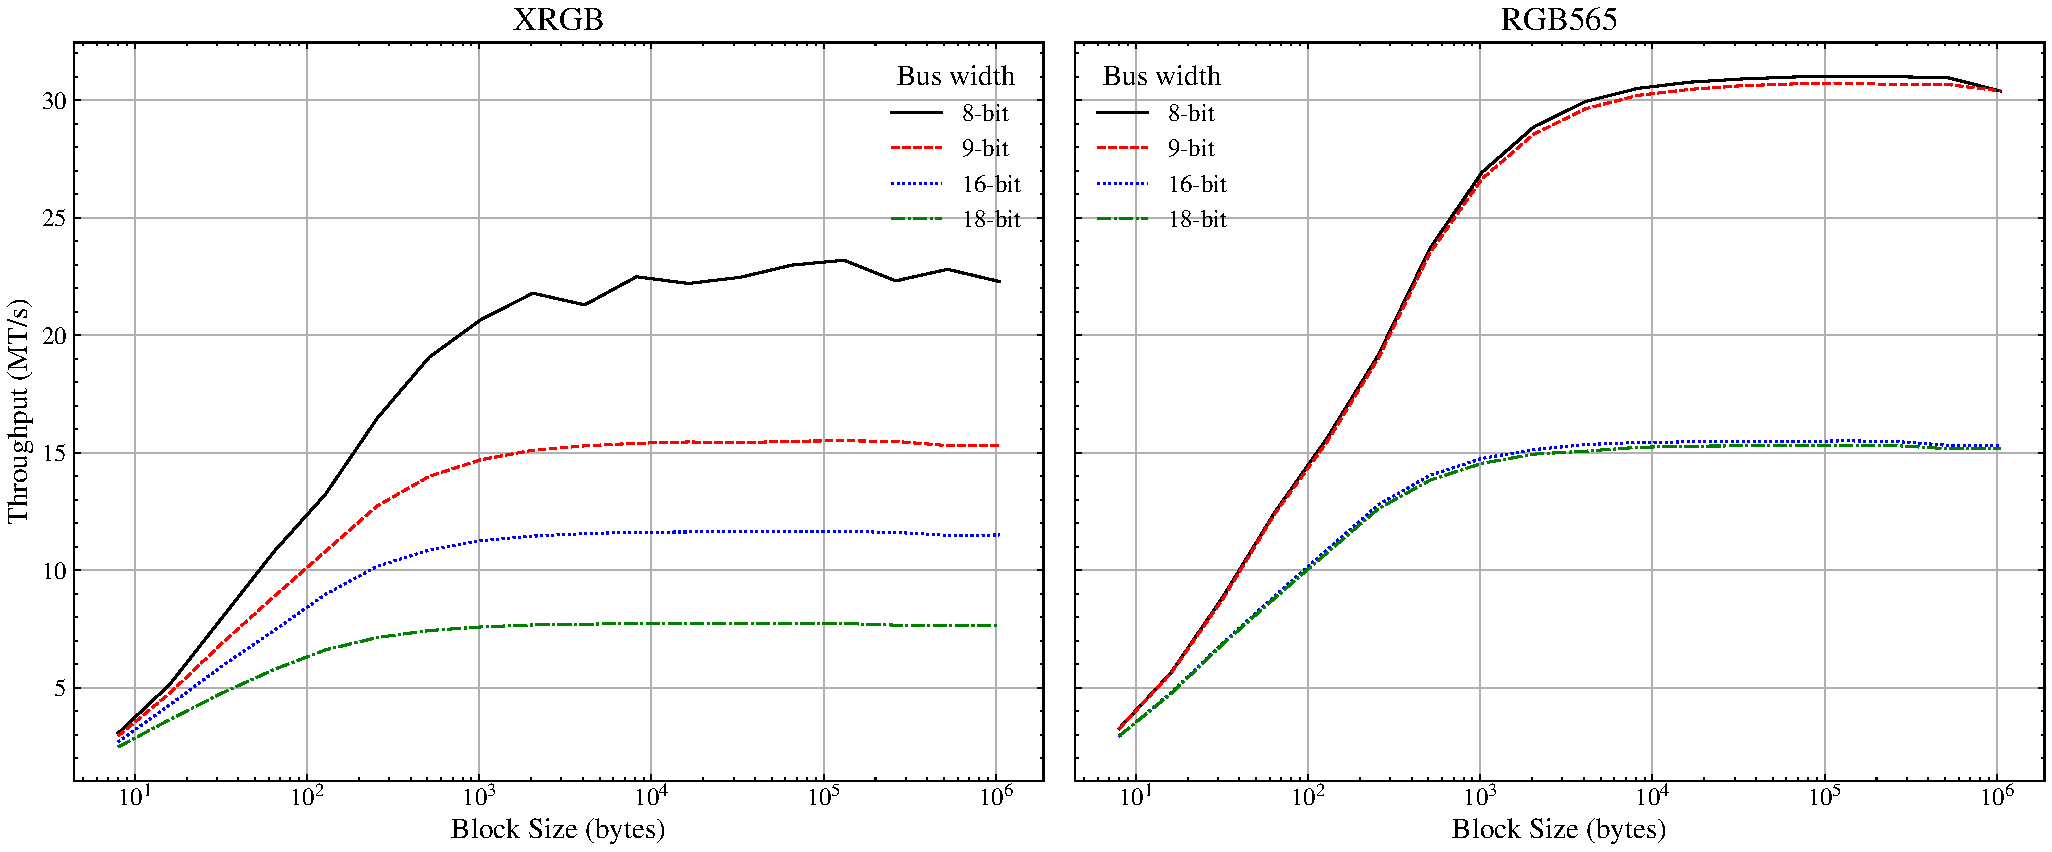
\includegraphics[width=1\textwidth]{img/rpi4-smi-throughput-mts.pdf}
\end{cmpfigure}

\begin{cmpfigure}[htb]{Raspberry Pi 4 SMI Throughput MB/s vs Block Size (O3, 64-bit OS)~\label{4_throughput_mbs}}
    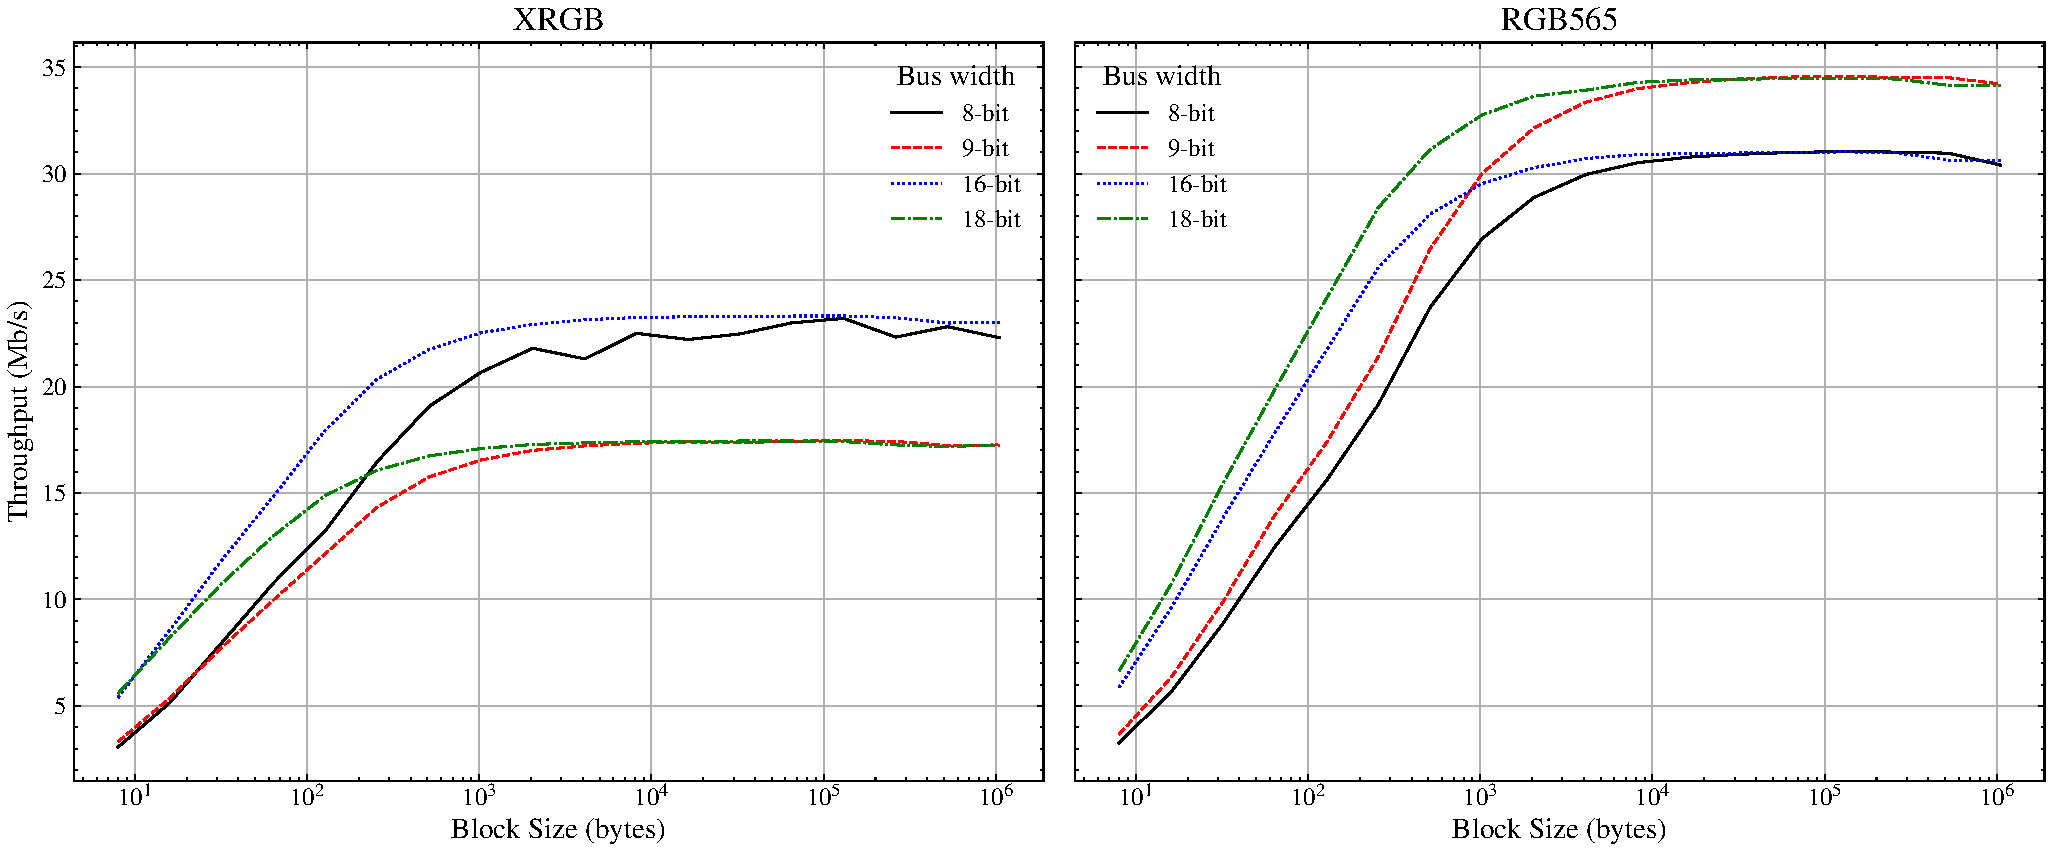
\includegraphics[width=1\textwidth]{img/rpi4-smi-throughput-mbs.pdf}
\end{cmpfigure}

\begin{cmpfigure}[htb]{Raspberry Pi 4 SMI Duration vs Block Size (O3, 64-bit OS)~\label{4_throughput_duration}}
    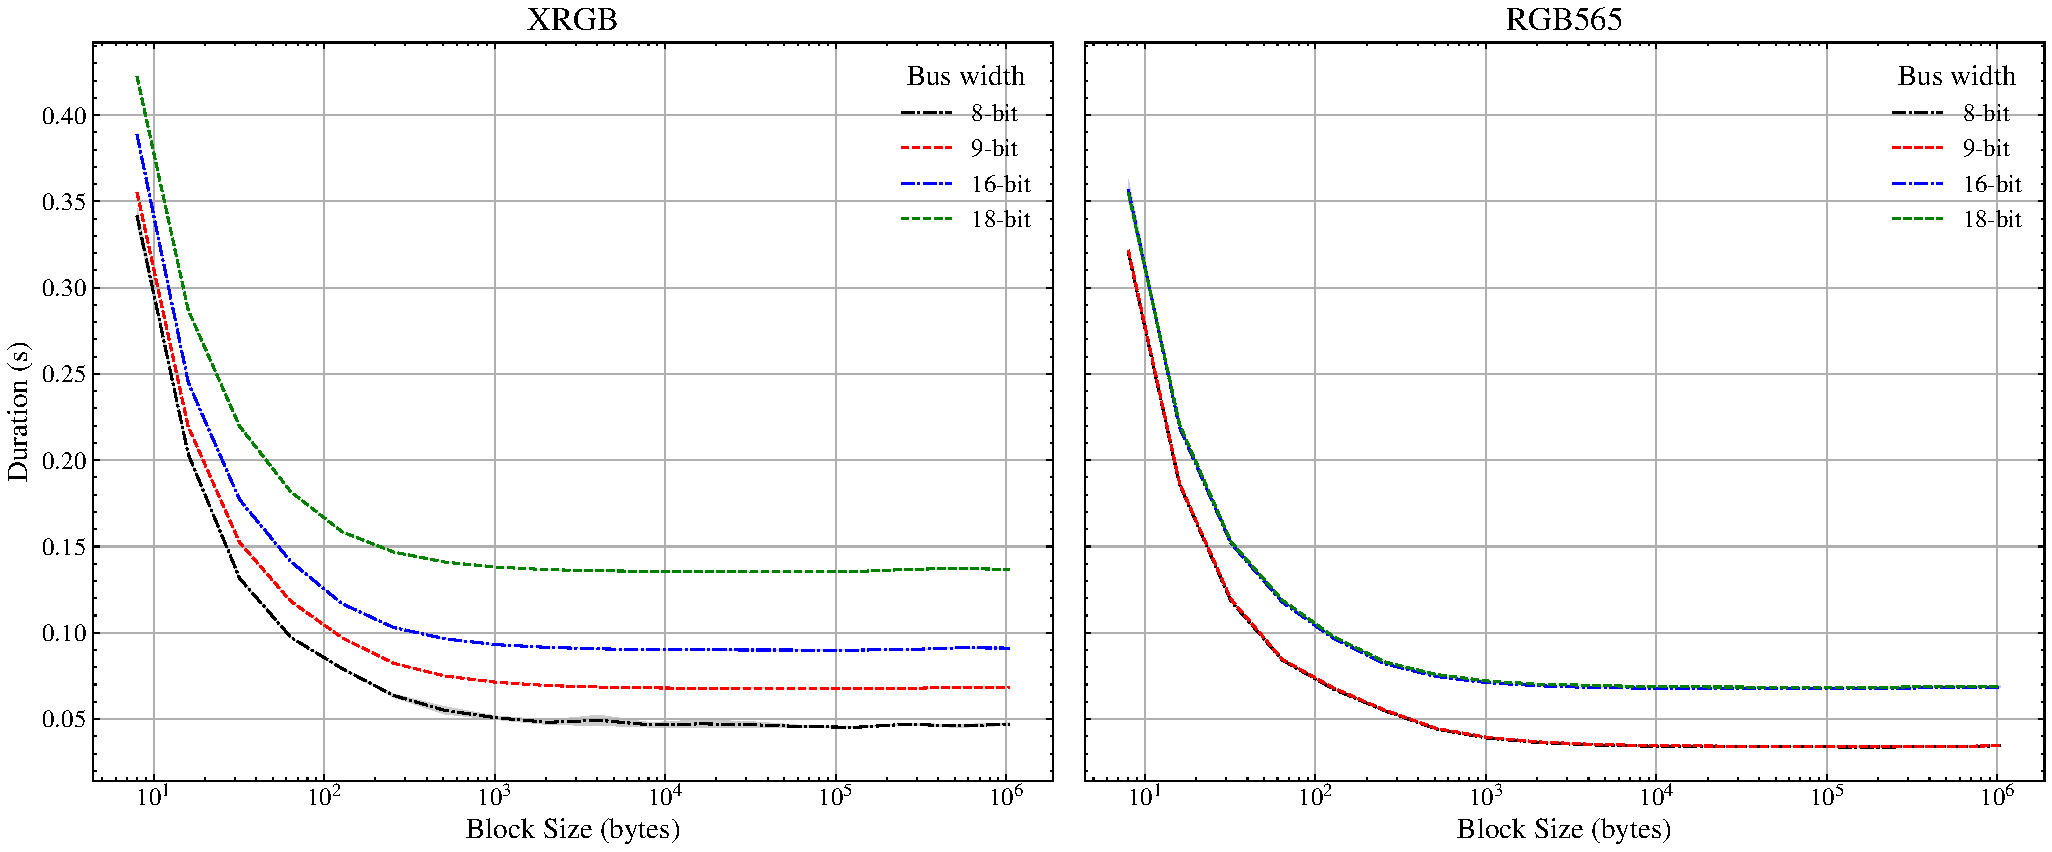
\includegraphics[width=1\textwidth]{img/rpi4-smi-duration.pdf}
\end{cmpfigure}

\begin{cmpfigure}[htb]{Raspberry Pi 3B+ SMI Data Cache Misses vs Block Size (O3, 32-bit OS)~\label{3b_cache_misses}}
    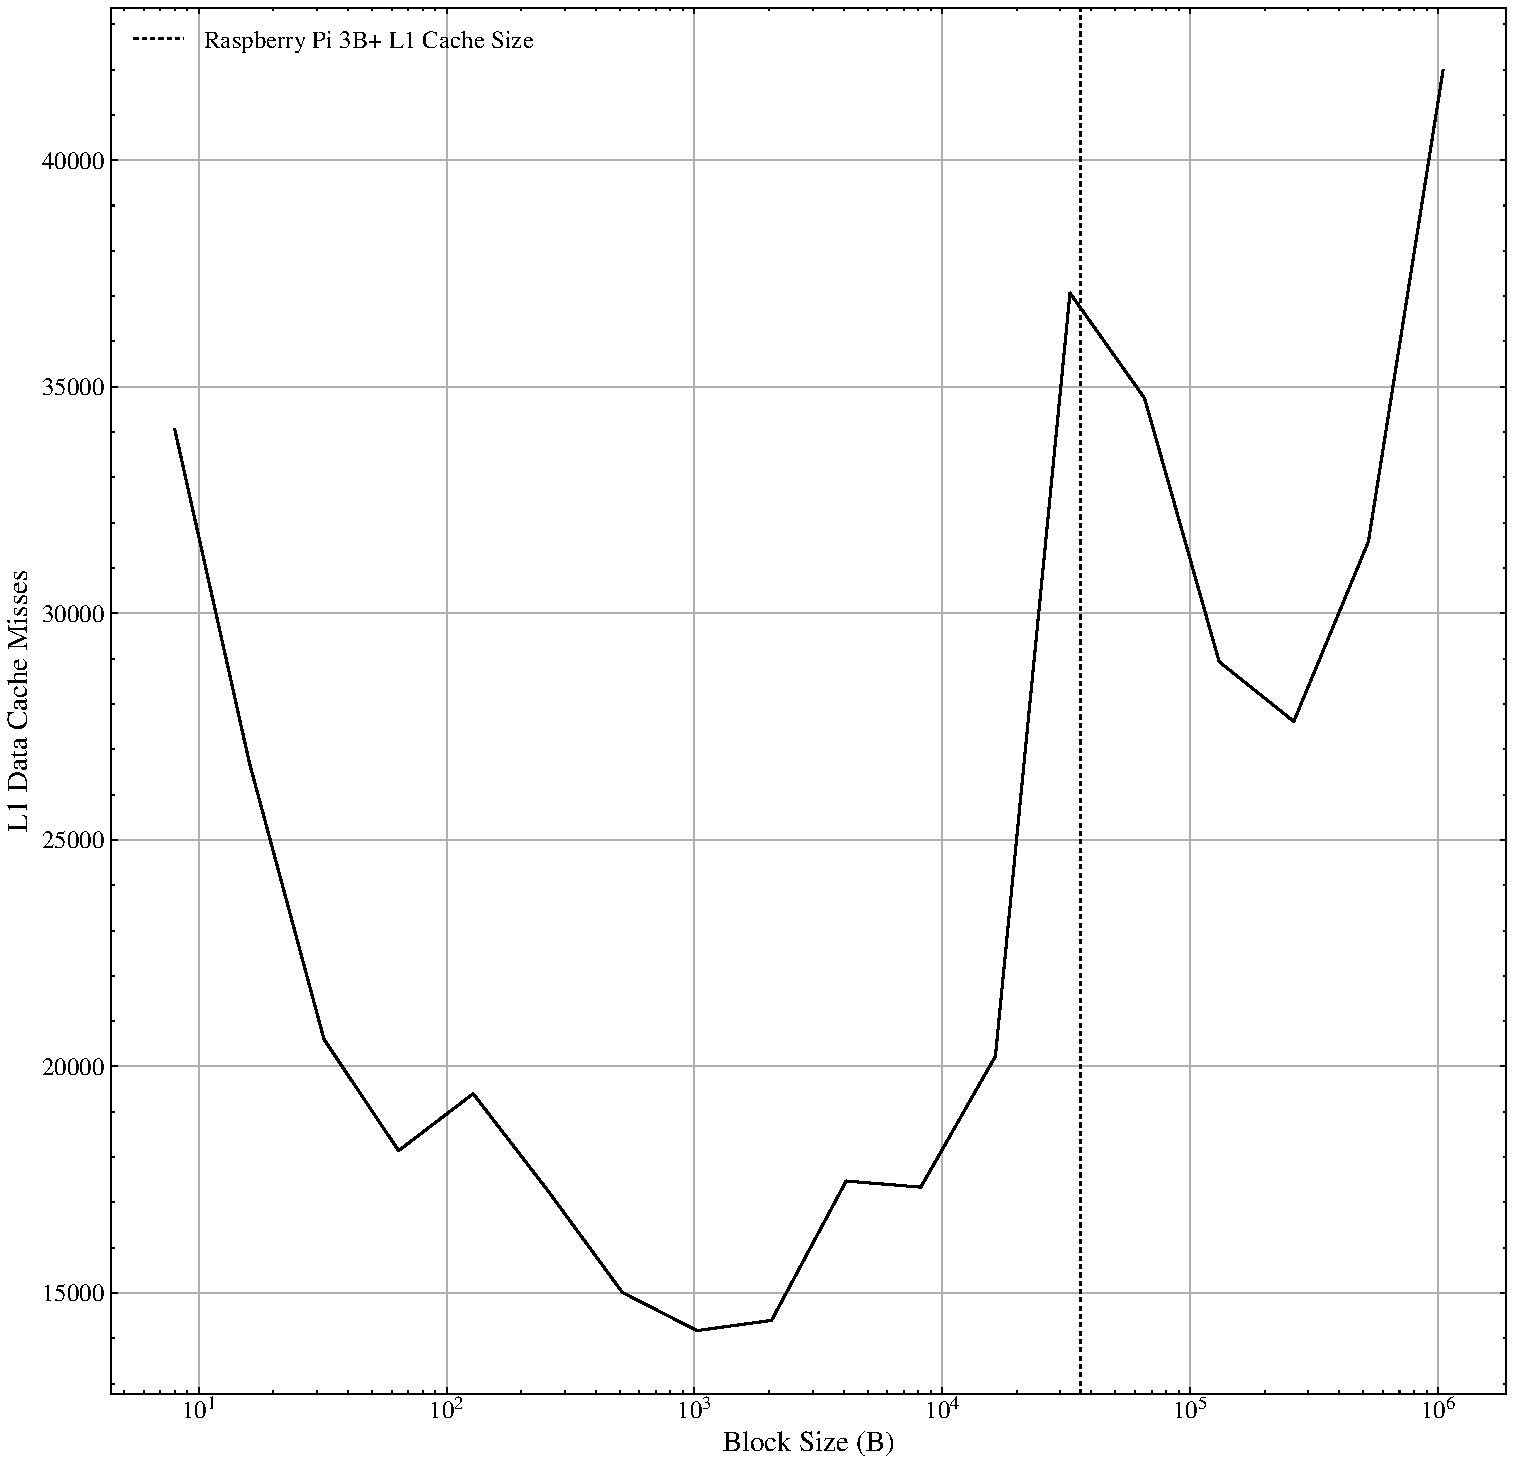
\includegraphics[width=1\textwidth]{img/rpi3b-smi-cache-misses.pdf}
\end{cmpfigure}

\begin{cmpfigure}[htb]{Raspberry Pi 3B+ SMI Data Cache Misses vs Throughput (MT/s) (O3, 32-bit OS)~\label{3b_cache_misses_throughput}}
    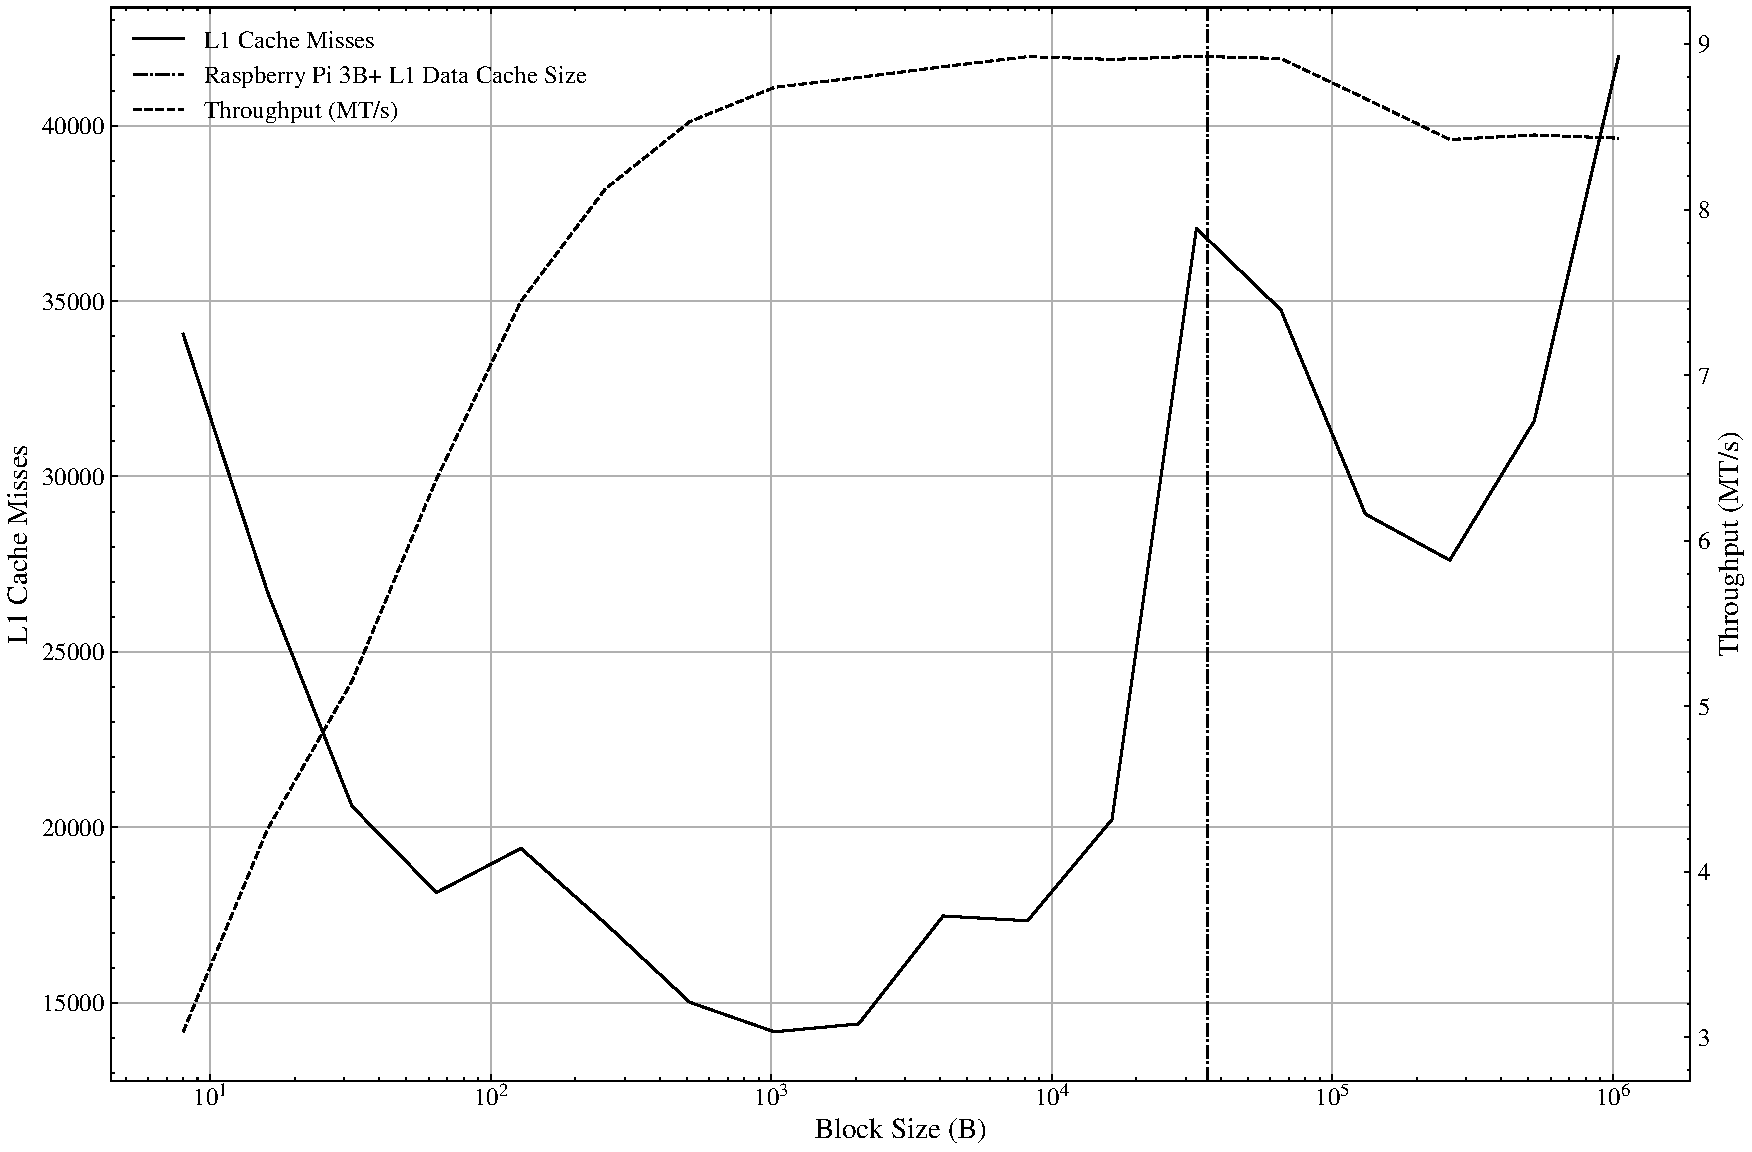
\includegraphics[width=1\textwidth]{img/rpi3b-smi-cache-misses-throughput.pdf}
\end{cmpfigure}



\clearpage
\section{Tables}

\begin{table}[h]
\centering
\label{tab:smi_dcs}
\begin{tabular}{|c|l|p{7cm}|c|c|}
\hline
\textbf{Bit(s)} & \textbf{Field} & \textbf{Description} & \textbf{Type} & \textbf{Reset} \\
\hline
31--4 & --- & Unused & - & - \\
\hline
3 & WRITE & Transfer Direction. 0 = Read from external device. 1 = Write to external device. & R/W & 0 \\
\hline
2 & DONE & Direct Transfer Complete. 0 = No meaning. 1 = Transfer has finished. Writing 1 clears this flag. & R/W & 0 \\
\hline
1 & START & Start Transfer. Writing 1 starts a transfer if one is not already in progress. & W & 0 \\
\hline
0 & ENABLE & Enable the SMI. OR'd with the ENABLE bit in SMI\_CS. 0 = Disable (power-saving state). 1 = Enable. & R/W & 0 \\
\hline
\end{tabular}
\caption{SMI Direct Control and Status Register (DCS)\label{dcs_register}}
\end{table}

\clearpage
\section{Gantt chart}\label{ApB}


\end{document}

